% Options for packages loaded elsewhere
% Options for packages loaded elsewhere
\PassOptionsToPackage{unicode}{hyperref}
\PassOptionsToPackage{hyphens}{url}
\PassOptionsToPackage{dvipsnames,svgnames,x11names}{xcolor}
%
\documentclass[
  russian,
  letterpaper,
  DIV=11,
  numbers=noendperiod]{scrartcl}
\usepackage{xcolor}
\usepackage{amsmath,amssymb}
\setcounter{secnumdepth}{5}
\usepackage{iftex}
\ifPDFTeX
  \usepackage[T1]{fontenc}
  \usepackage[utf8]{inputenc}
  \usepackage{textcomp} % provide euro and other symbols
\else % if luatex or xetex
  \usepackage{unicode-math} % this also loads fontspec
  \defaultfontfeatures{Scale=MatchLowercase}
  \defaultfontfeatures[\rmfamily]{Ligatures=TeX,Scale=1}
\fi
\usepackage{lmodern}
\ifPDFTeX\else
  % xetex/luatex font selection
\fi
% Use upquote if available, for straight quotes in verbatim environments
\IfFileExists{upquote.sty}{\usepackage{upquote}}{}
\IfFileExists{microtype.sty}{% use microtype if available
  \usepackage[]{microtype}
  \UseMicrotypeSet[protrusion]{basicmath} % disable protrusion for tt fonts
}{}
\makeatletter
\@ifundefined{KOMAClassName}{% if non-KOMA class
  \IfFileExists{parskip.sty}{%
    \usepackage{parskip}
  }{% else
    \setlength{\parindent}{0pt}
    \setlength{\parskip}{6pt plus 2pt minus 1pt}}
}{% if KOMA class
  \KOMAoptions{parskip=half}}
\makeatother
% Make \paragraph and \subparagraph free-standing
\makeatletter
\ifx\paragraph\undefined\else
  \let\oldparagraph\paragraph
  \renewcommand{\paragraph}{
    \@ifstar
      \xxxParagraphStar
      \xxxParagraphNoStar
  }
  \newcommand{\xxxParagraphStar}[1]{\oldparagraph*{#1}\mbox{}}
  \newcommand{\xxxParagraphNoStar}[1]{\oldparagraph{#1}\mbox{}}
\fi
\ifx\subparagraph\undefined\else
  \let\oldsubparagraph\subparagraph
  \renewcommand{\subparagraph}{
    \@ifstar
      \xxxSubParagraphStar
      \xxxSubParagraphNoStar
  }
  \newcommand{\xxxSubParagraphStar}[1]{\oldsubparagraph*{#1}\mbox{}}
  \newcommand{\xxxSubParagraphNoStar}[1]{\oldsubparagraph{#1}\mbox{}}
\fi
\makeatother

\usepackage{color}
\usepackage{fancyvrb}
\newcommand{\VerbBar}{|}
\newcommand{\VERB}{\Verb[commandchars=\\\{\}]}
\DefineVerbatimEnvironment{Highlighting}{Verbatim}{commandchars=\\\{\}}
% Add ',fontsize=\small' for more characters per line
\usepackage{framed}
\definecolor{shadecolor}{RGB}{241,243,245}
\newenvironment{Shaded}{\begin{snugshade}}{\end{snugshade}}
\newcommand{\AlertTok}[1]{\textcolor[rgb]{0.68,0.00,0.00}{#1}}
\newcommand{\AnnotationTok}[1]{\textcolor[rgb]{0.37,0.37,0.37}{#1}}
\newcommand{\AttributeTok}[1]{\textcolor[rgb]{0.40,0.45,0.13}{#1}}
\newcommand{\BaseNTok}[1]{\textcolor[rgb]{0.68,0.00,0.00}{#1}}
\newcommand{\BuiltInTok}[1]{\textcolor[rgb]{0.00,0.23,0.31}{#1}}
\newcommand{\CharTok}[1]{\textcolor[rgb]{0.13,0.47,0.30}{#1}}
\newcommand{\CommentTok}[1]{\textcolor[rgb]{0.37,0.37,0.37}{#1}}
\newcommand{\CommentVarTok}[1]{\textcolor[rgb]{0.37,0.37,0.37}{\textit{#1}}}
\newcommand{\ConstantTok}[1]{\textcolor[rgb]{0.56,0.35,0.01}{#1}}
\newcommand{\ControlFlowTok}[1]{\textcolor[rgb]{0.00,0.23,0.31}{\textbf{#1}}}
\newcommand{\DataTypeTok}[1]{\textcolor[rgb]{0.68,0.00,0.00}{#1}}
\newcommand{\DecValTok}[1]{\textcolor[rgb]{0.68,0.00,0.00}{#1}}
\newcommand{\DocumentationTok}[1]{\textcolor[rgb]{0.37,0.37,0.37}{\textit{#1}}}
\newcommand{\ErrorTok}[1]{\textcolor[rgb]{0.68,0.00,0.00}{#1}}
\newcommand{\ExtensionTok}[1]{\textcolor[rgb]{0.00,0.23,0.31}{#1}}
\newcommand{\FloatTok}[1]{\textcolor[rgb]{0.68,0.00,0.00}{#1}}
\newcommand{\FunctionTok}[1]{\textcolor[rgb]{0.28,0.35,0.67}{#1}}
\newcommand{\ImportTok}[1]{\textcolor[rgb]{0.00,0.46,0.62}{#1}}
\newcommand{\InformationTok}[1]{\textcolor[rgb]{0.37,0.37,0.37}{#1}}
\newcommand{\KeywordTok}[1]{\textcolor[rgb]{0.00,0.23,0.31}{\textbf{#1}}}
\newcommand{\NormalTok}[1]{\textcolor[rgb]{0.00,0.23,0.31}{#1}}
\newcommand{\OperatorTok}[1]{\textcolor[rgb]{0.37,0.37,0.37}{#1}}
\newcommand{\OtherTok}[1]{\textcolor[rgb]{0.00,0.23,0.31}{#1}}
\newcommand{\PreprocessorTok}[1]{\textcolor[rgb]{0.68,0.00,0.00}{#1}}
\newcommand{\RegionMarkerTok}[1]{\textcolor[rgb]{0.00,0.23,0.31}{#1}}
\newcommand{\SpecialCharTok}[1]{\textcolor[rgb]{0.37,0.37,0.37}{#1}}
\newcommand{\SpecialStringTok}[1]{\textcolor[rgb]{0.13,0.47,0.30}{#1}}
\newcommand{\StringTok}[1]{\textcolor[rgb]{0.13,0.47,0.30}{#1}}
\newcommand{\VariableTok}[1]{\textcolor[rgb]{0.07,0.07,0.07}{#1}}
\newcommand{\VerbatimStringTok}[1]{\textcolor[rgb]{0.13,0.47,0.30}{#1}}
\newcommand{\WarningTok}[1]{\textcolor[rgb]{0.37,0.37,0.37}{\textit{#1}}}

\usepackage{longtable,booktabs,array}
\usepackage{calc} % for calculating minipage widths
% Correct order of tables after \paragraph or \subparagraph
\usepackage{etoolbox}
\makeatletter
\patchcmd\longtable{\par}{\if@noskipsec\mbox{}\fi\par}{}{}
\makeatother
% Allow footnotes in longtable head/foot
\IfFileExists{footnotehyper.sty}{\usepackage{footnotehyper}}{\usepackage{footnote}}
\makesavenoteenv{longtable}
\usepackage{graphicx}
\makeatletter
\newsavebox\pandoc@box
\newcommand*\pandocbounded[1]{% scales image to fit in text height/width
  \sbox\pandoc@box{#1}%
  \Gscale@div\@tempa{\textheight}{\dimexpr\ht\pandoc@box+\dp\pandoc@box\relax}%
  \Gscale@div\@tempb{\linewidth}{\wd\pandoc@box}%
  \ifdim\@tempb\p@<\@tempa\p@\let\@tempa\@tempb\fi% select the smaller of both
  \ifdim\@tempa\p@<\p@\scalebox{\@tempa}{\usebox\pandoc@box}%
  \else\usebox{\pandoc@box}%
  \fi%
}
% Set default figure placement to htbp
\def\fps@figure{htbp}
\makeatother



\ifLuaTeX
\usepackage[bidi=basic,provide=*]{babel}
\else
\usepackage[bidi=default,provide=*]{babel}
\fi
% get rid of language-specific shorthands (see #6817):
\let\LanguageShortHands\languageshorthands
\def\languageshorthands#1{}


\setlength{\emergencystretch}{3em} % prevent overfull lines

\providecommand{\tightlist}{%
  \setlength{\itemsep}{0pt}\setlength{\parskip}{0pt}}



 


\usepackage{fontspec}

\setsansfont{Palatino Linotype}[
    Path=../files/palatino/,
    Extension = .ttf,
    UprightFont=palatino-Roman,
    BoldFont=palatino-Bold,
    ItalicFont=palatino-Italic,
    BoldItalicFont=palatino-BoldItalic
]
\setmainfont{Palatino Linotype}[
    Path=../files/palatino/,
    Extension = .ttf,
    UprightFont=palatino-Roman,
    BoldFont=palatino-Bold,
    ItalicFont=palatino-Italic,
    BoldItalicFont=palatino-BoldItalic
]

\usepackage[textwidth=0.86\paperwidth, textheight=0.86\paperheight]{geometry}
\usepackage{fancyhdr}
\usepackage{hyperref}
\usepackage{fontawesome5}
\usepackage{graphicx}
\usepackage{amssymb}
\usepackage{amsmath}
\graphicspath{{../files/}}

\newcommand{\R}{\mathbb{R}}

% \pagenumbering{gobble}
\pagestyle{fancy}
\fancyhead{} % clear all header fields
\fancyhead[R]{\href{https://cu25.fmin.xyz}{\faGem[regular]} \hspace{0.04cm} \href{https://github.com/MerkulovDaniil/cu25}{\faGithub} \hspace{0.07cm} \href{https://t.me/fminxyz}{\faTelegram}}
\fancyhead[L]{\href{https://fmin.xyz}{
\includegraphics[height=0.35cm]{logo.pdf}} \hspace{2pt} \textbf{Оптимизация для всех! ЦУ. 2025}}
\KOMAoption{captions}{tableheading}
\makeatletter
\@ifpackageloaded{tcolorbox}{}{\usepackage[skins,breakable]{tcolorbox}}
\@ifpackageloaded{fontawesome5}{}{\usepackage{fontawesome5}}
\definecolor{quarto-callout-color}{HTML}{909090}
\definecolor{quarto-callout-note-color}{HTML}{0758E5}
\definecolor{quarto-callout-important-color}{HTML}{CC1914}
\definecolor{quarto-callout-warning-color}{HTML}{EB9113}
\definecolor{quarto-callout-tip-color}{HTML}{00A047}
\definecolor{quarto-callout-caution-color}{HTML}{FC5300}
\definecolor{quarto-callout-color-frame}{HTML}{acacac}
\definecolor{quarto-callout-note-color-frame}{HTML}{4582ec}
\definecolor{quarto-callout-important-color-frame}{HTML}{d9534f}
\definecolor{quarto-callout-warning-color-frame}{HTML}{f0ad4e}
\definecolor{quarto-callout-tip-color-frame}{HTML}{02b875}
\definecolor{quarto-callout-caution-color-frame}{HTML}{fd7e14}
\makeatother
\makeatletter
\@ifpackageloaded{caption}{}{\usepackage{caption}}
\AtBeginDocument{%
\ifdefined\contentsname
  \renewcommand*\contentsname{Содержание}
\else
  \newcommand\contentsname{Содержание}
\fi
\ifdefined\listfigurename
  \renewcommand*\listfigurename{Список Иллюстраций}
\else
  \newcommand\listfigurename{Список Иллюстраций}
\fi
\ifdefined\listtablename
  \renewcommand*\listtablename{Список Таблиц}
\else
  \newcommand\listtablename{Список Таблиц}
\fi
\ifdefined\figurename
  \renewcommand*\figurename{Рисунок}
\else
  \newcommand\figurename{Рисунок}
\fi
\ifdefined\tablename
  \renewcommand*\tablename{Таблица}
\else
  \newcommand\tablename{Таблица}
\fi
}
\@ifpackageloaded{float}{}{\usepackage{float}}
\floatstyle{ruled}
\@ifundefined{c@chapter}{\newfloat{codelisting}{h}{lop}}{\newfloat{codelisting}{h}{lop}[chapter]}
\floatname{codelisting}{Список}
\newcommand*\listoflistings{\listof{codelisting}{Список Каталогов}}
\makeatother
\makeatletter
\makeatother
\makeatletter
\@ifpackageloaded{caption}{}{\usepackage{caption}}
\@ifpackageloaded{subcaption}{}{\usepackage{subcaption}}
\makeatother
\usepackage{bookmark}
\IfFileExists{xurl.sty}{\usepackage{xurl}}{} % add URL line breaks if available
\urlstyle{same}
\hypersetup{
  pdftitle={Автоматическое дифференцирование},
  pdfauthor={Даня Меркулов},
  pdflang={ru},
  colorlinks=true,
  linkcolor={blue},
  filecolor={Maroon},
  citecolor={Blue},
  urlcolor={Blue},
  pdfcreator={LaTeX via pandoc}}


\title{Автоматическое дифференцирование}
\author{Даня Меркулов}
\date{}
\begin{document}
\maketitle


\section{Автоматическое
дифференцирование}\label{ux430ux432ux442ux43eux43cux430ux442ux438ux447ux435ux441ux43aux43eux435-ux434ux438ux444ux444ux435ux440ux435ux43dux446ux438ux440ux43eux432ux430ux43dux438ux435}

\begin{figure}[H]

{\centering \pandocbounded{
\includegraphics[keepaspectratio]{autograd_expectations.jpeg}}

}

\caption{Когда вы поняли идею}

\end{figure}%

\begin{figure}[H]

{\centering 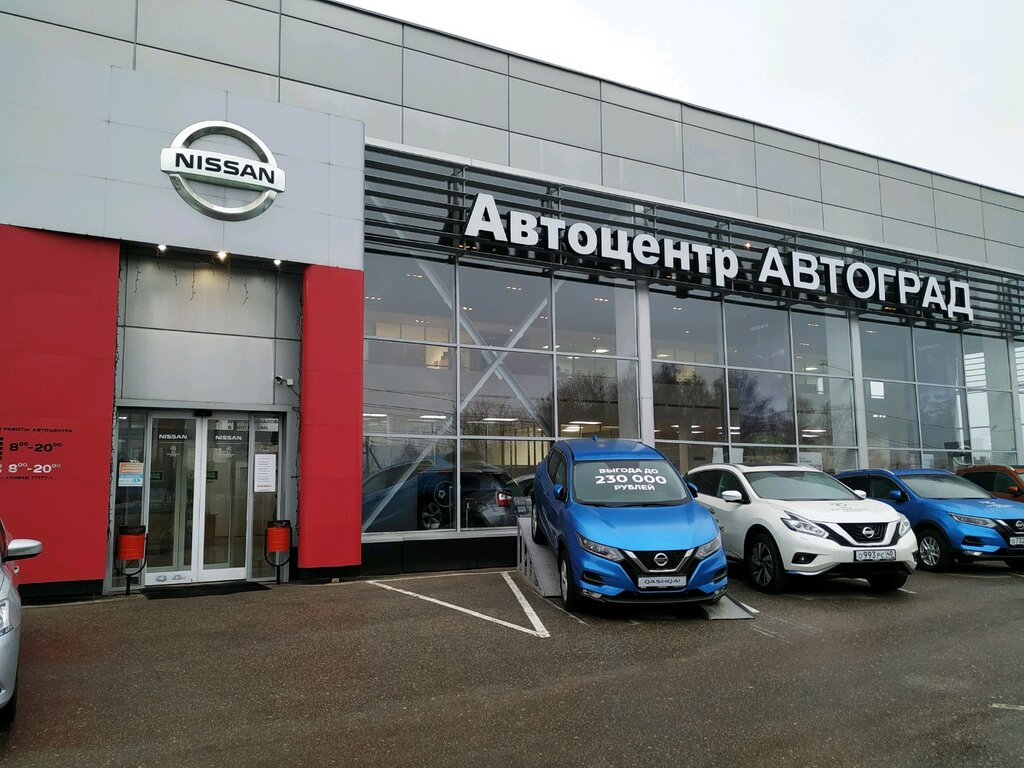
\includegraphics[width=0.65\linewidth,height=\textheight,keepaspectratio]{avtograd.jpeg}

}

\caption{Это не autograd}

\end{figure}%

\subsection{Задача}\label{ux437ux430ux434ux430ux447ux430}

Предположим, что мы хотим решить следующую задачу: \[
L(w) \to \min_{w \in \mathbb{R}^d}
\]

\begin{itemize}
\tightlist
\item
  Такие задачи обычно возникают в машинном обучении, когда нам нужно
  найти подходящие параметры \(w\) модели (например, обучить нейронную
  сеть).
\item
  Существуют разные методы решения этой задачи. Однако, размерность
  задач сегодня может достигать сотен миллиардов или даже триллионов
  переменных. Такие задачи очень тяжело решать без знания градиентов, то
  есть методами нулевого порядка.
\item
  Поэтому было бы полезно уметь вычислять вектор градиента
  \(\nabla_w L = \left( \frac{\partial L}{\partial w_1}, \ldots, \frac{\partial L}{\partial w_d}\right)^T\).
\item
  Обычно методы первого порядка работают лучше в больших задачах, в то
  время как методы второго порядка требуют слишком много памяти.
\end{itemize}

\subsection{Задача многомерного
шкалирования}\label{ux437ux430ux434ux430ux447ux430-ux43cux43dux43eux433ux43eux43cux435ux440ux43dux43eux433ux43e-ux448ux43aux430ux43bux438ux440ux43eux432ux430ux43dux438ux44f}

Предположим, что у нас есть матрица расстояний для \(N\) \(d\)-мерных
объектов \(D \in \mathbb{R}^{N \times N}\). Используя эту матрицу, мы
хотим восстановить исходные координаты
\(W_i \in \mathbb{R}^d, \; i = 1, \ldots, N\).

\[
L(W) = \sum_{i, j = 1}^N \left(\|W_i - W_j\|^2_2 - D_{i,j}\right)^2 \to \min_{W \in \mathbb{R}^{N \times d}}
\]

Ссылка на визуализацию
\href{http://www.benfrederickson.com/numerical-optimization/}{\(\clubsuit\)},
где можно увидеть, что безградиентные методы оптимизации решают эту
задачу намного медленнее, особенно в пространствах большой размерности.

\begin{tcolorbox}[enhanced jigsaw, colframe=quarto-callout-color-frame, rightrule=.15mm, toprule=.15mm, coltitle=black, opacityback=0, colback=white, leftrule=.75mm, arc=.35mm, opacitybacktitle=0.6, bottomrule=.15mm, breakable, toptitle=1mm, colbacktitle=quarto-callout-color!10!white, bottomtitle=1mm, title=\textcolor{quarto-callout-color}{\faInfo}\hspace{0.5em}{Question}, left=2mm, titlerule=0mm]

Связано ли это с PCA?

\end{tcolorbox}

\begin{figure}[H]

{\centering 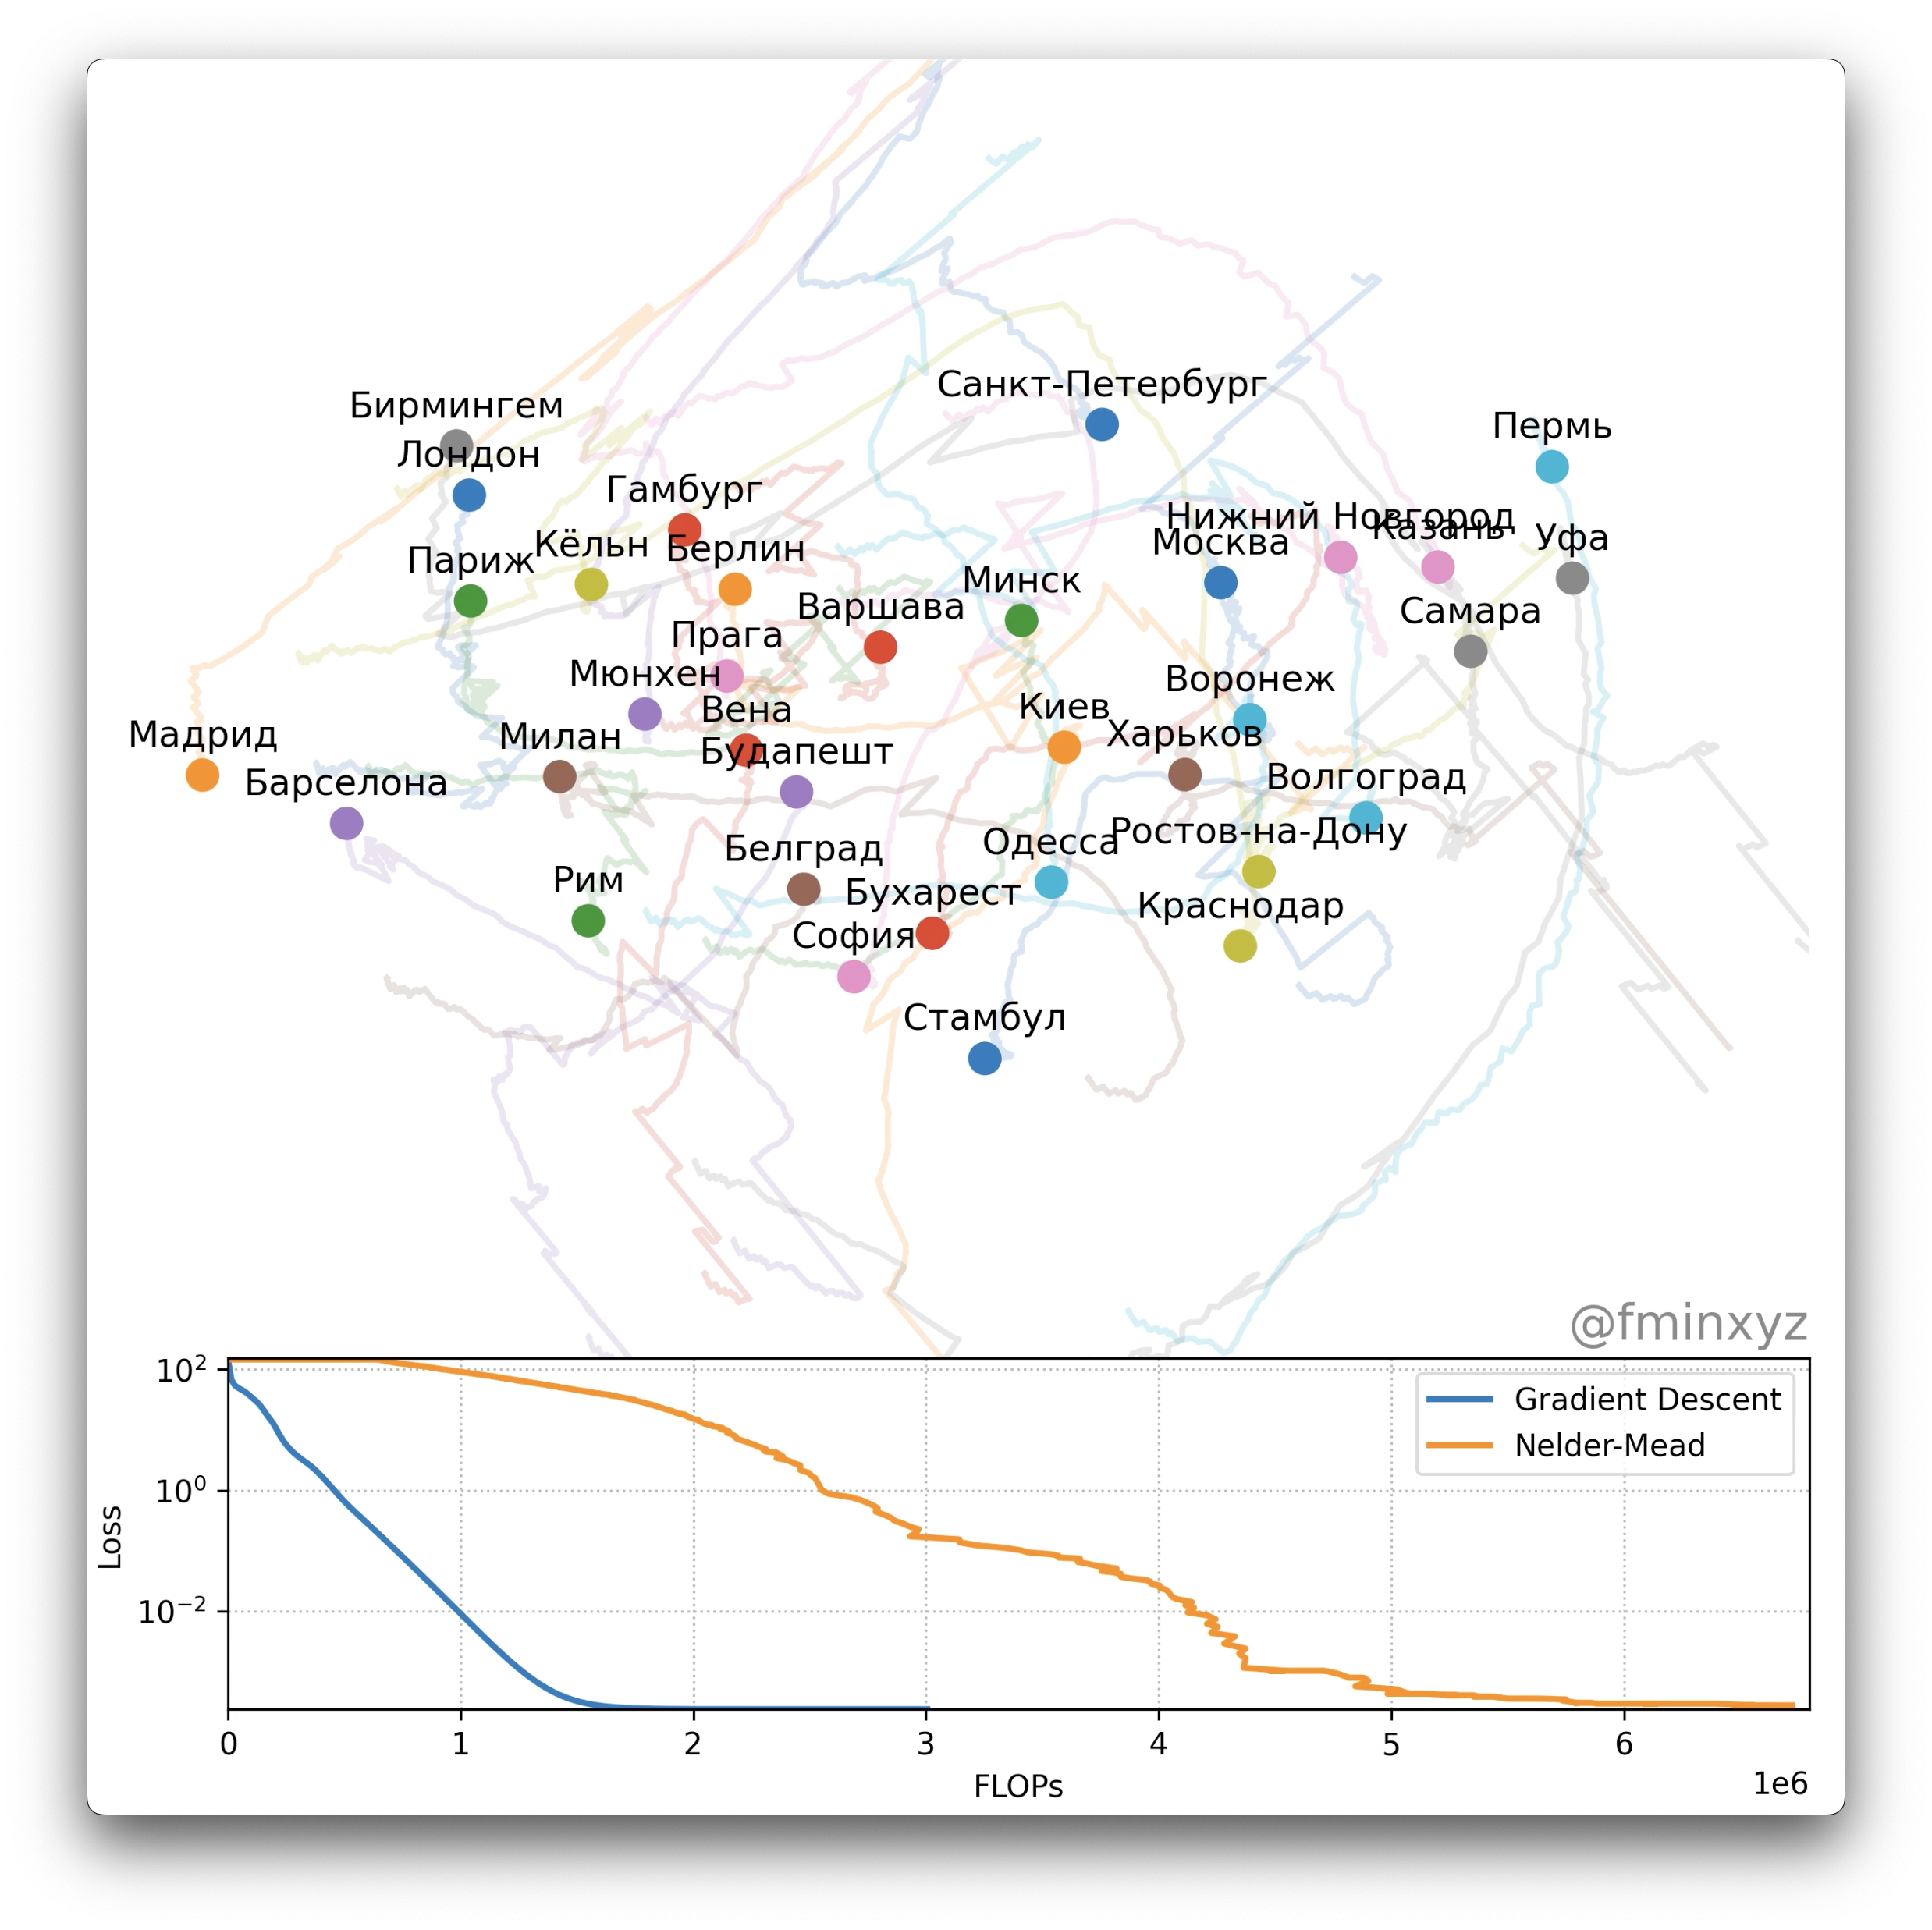
\includegraphics[width=0.4\linewidth,height=\textheight,keepaspectratio]{mds.png}

}

\caption{\href{https://fmin.xyz/docs/visualizations/mds.mp4}{Ссылка на
анимацию}}

\end{figure}%

\subsection{Градиентный спуск без
градиента}\label{ux433ux440ux430ux434ux438ux435ux43dux442ux43dux44bux439-ux441ux43fux443ux441ux43a-ux431ux435ux437-ux433ux440ux430ux434ux438ux435ux43dux442ux430}

Предположим, что мы хотим решить следующую задачу: \[
L(w) \to \min_{w \in \mathbb{R}^d}
\]

с помощью алгоритма градиентного спуска (GD): \[
w_{k+1} = w_k - \alpha_k \nabla_w L(w_k)
\]

Можно ли заменить \(\nabla_w L(w_k)\) используя только информацию
нулевого порядка?

Да, но за определенную цену.

Рассмотрим двухточечную оценку градиента\footnote{рекомендуется
  \href{https://scholar.harvard.edu/files/yujietang/files/slides_2019_zero-order_opt_tutorial.pdf}{хорошая}
  презентация о безградиентных методах} \(G\): \[
G = d\dfrac{L(w + \varepsilon v)- L(w - \varepsilon v)}{2 \varepsilon}v, 
\] где \(v\) сферически симметричен.

\begin{figure}[H]

{\centering 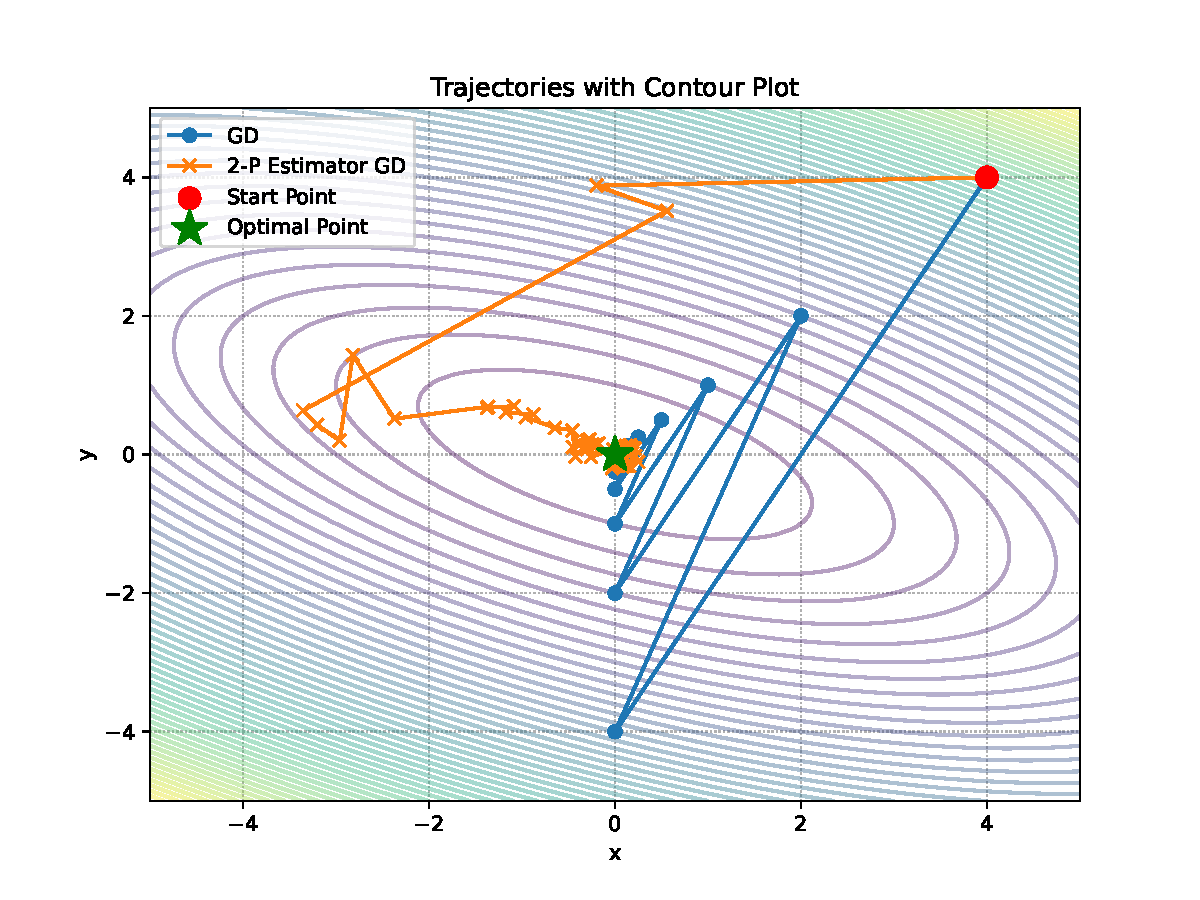
\includegraphics[width=0.8\linewidth,height=\textheight,keepaspectratio]{zgd_2p.pdf}

}

\caption{``Иллюстрация двухточечной оценки градиентного спуска''}

\end{figure}%

\subsection{Конечные
разности}\label{ux43aux43eux43dux435ux447ux43dux44bux435-ux440ux430ux437ux43dux43eux441ux442ux438}

\[
w_{k+1} = w_k - \alpha_k G
\]

Также рассмотрим идею конечных разностей: \[
G =  \sum\limits_{i=1}^d\dfrac{L(w+\varepsilon e_i) - L(w-\varepsilon e_i)}{2\varepsilon} e_i
\]
\href{https://colab.research.google.com/github/MerkulovDaniil/optim/blob/master/assets/Notebooks/Zero_order_GD.ipynb}{Открыть
в Colab \(\clubsuit\)}

\begin{figure}[H]

{\centering 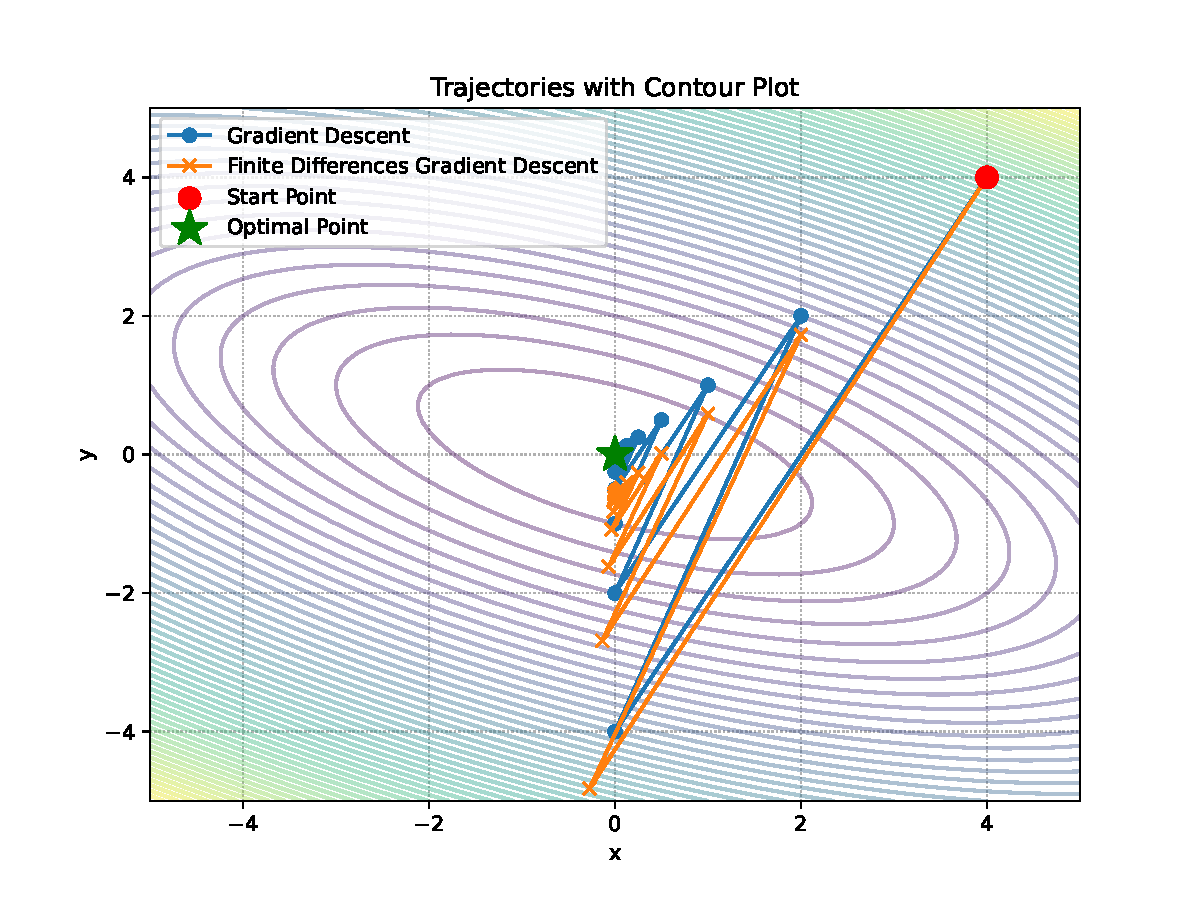
\includegraphics[width=0.8\linewidth,height=\textheight,keepaspectratio]{zgd_fd.pdf}

}

\caption{``Иллюстрация работы метода оценки градиента с помощью метода
конечных разностей''}

\end{figure}%

\subsection[Проклятие размерности для методов нулевого порядка
]{\texorpdfstring{Проклятие размерности для методов нулевого порядка
\footnote{\href{https://arxiv.org/pdf/1312.2139}{Оптимальные скорости
  для нулевого порядка выпуклой оптимизации: сила двух оценок функции}}}{Проклятие размерности для методов нулевого порядка }}\label{ux43fux440ux43eux43aux43bux44fux442ux438ux435-ux440ux430ux437ux43cux435ux440ux43dux43eux441ux442ux438-ux434ux43bux44f-ux43cux435ux442ux43eux434ux43eux432-ux43dux443ux43bux435ux432ux43eux433ux43e-ux43fux43eux440ux44fux434ux43aux430}

\[
\min_{x \in \mathbb{R}^n} f(x)
\]

\[
\text{GD: } x_{k+1} = x_k - \alpha_k \nabla f(x_k) \qquad \qquad \text{Zero order GD: } x_{k+1} = x_k - \alpha_k G,
\]

где \(G\) - оценка градиента 2-точечная или многоточечная.

\begin{longtable}[]{@{}
  >{\centering\arraybackslash}p{(\linewidth - 6\tabcolsep) * \real{0.1304}}
  >{\centering\arraybackslash}p{(\linewidth - 6\tabcolsep) * \real{0.2174}}
  >{\centering\arraybackslash}p{(\linewidth - 6\tabcolsep) * \real{0.2609}}
  >{\centering\arraybackslash}p{(\linewidth - 6\tabcolsep) * \real{0.3913}}@{}}
\toprule\noalign{}
\begin{minipage}[b]{\linewidth}\centering
\end{minipage} & \begin{minipage}[b]{\linewidth}\centering
\(f(x)\) - гладкая
\end{minipage} & \begin{minipage}[b]{\linewidth}\centering
\(f(x)\) - гладкая и выпуклая
\end{minipage} & \begin{minipage}[b]{\linewidth}\centering
\(f(x)\) - гладкая и сильно выпуклая
\end{minipage} \\
\midrule\noalign{}
\endhead
\bottomrule\noalign{}
\endlastfoot
GD &
\(\|\nabla f(x_k)\|^2 \approx \mathcal{O} \left( \dfrac{1}{k} \right)\)
& \(f(x_k) - f^* \approx  \mathcal{O} \left( \dfrac{1}{k} \right)\) &
\(\|x_k - x^*\|^2 \approx \mathcal{O} \left( \left(1 - \dfrac{\mu}{L}\right)^k \right)\) \\
GD нулевого порядка &
\(\|\nabla f(x_k)\|^2 \approx \mathcal{O} \left( \dfrac{n}{k} \right)\)
& \(f(x_k) - f^* \approx  \mathcal{O} \left( \dfrac{n}{k} \right)\) &
\(\|x_k - x^*\|^2 \approx \mathcal{O} \left( \left(1 - \dfrac{\mu}{n L}\right)^k \right)\) \\
\end{longtable}

Для 2-точечных оценок, мы не можем сделать зависимость лучше, чем от
\(\sqrt{n}\) !

\subsection{Конечные
разности}\label{ux43aux43eux43dux435ux447ux43dux44bux435-ux440ux430ux437ux43dux43eux441ux442ux438-1}

Наивный подход к получению приблизительных значений градиентов - это
подход \textbf{конечных разностей}. Для каждой координаты, можно
вычислить приближенное значение частной производной: \[
\dfrac{\partial L}{\partial w_k} (w) \approx \dfrac{L(w+\varepsilon e_k) - L(w)}{\varepsilon}, \quad e_k = (0, \ldots, \underset{{\tiny k}}{1}, \ldots, 0)
\]

\begin{tcolorbox}[enhanced jigsaw, colframe=quarto-callout-color-frame, rightrule=.15mm, toprule=.15mm, coltitle=black, opacityback=0, colback=white, leftrule=.75mm, arc=.35mm, opacitybacktitle=0.6, bottomrule=.15mm, breakable, toptitle=1mm, colbacktitle=quarto-callout-color!10!white, bottomtitle=1mm, title=\textcolor{quarto-callout-color}{\faInfo}\hspace{0.5em}{Question}, left=2mm, titlerule=0mm]

Если время, необходимое для одного вычисления \(L(w)\) равно \(T\), то
какое время необходимо для вычисления \(\nabla_w L\) с этим подходом?

\textbf{Ответ} \(2dT\), что очень долго для больших задач. Кроме того,
этот метод нестабилен, что означает, что нам придется выбирать между
точностью и стабильностью.

\textbf{Теорема}

Существует алгоритм для вычисления \(\nabla_w L\) за \(\mathcal{O}(T)\).
\footnotemark{}

\end{tcolorbox}

\footnotetext{Linnainmaa S. The representation of the cumulative
rounding error of an algorithm as a Taylor expansion of the local
rounding errors. Master's Thesis (in Finnish), Univ. Helsinki, 1970.}

\subsection{Прямой режим автоматического
дифференцирования}\label{ux43fux440ux44fux43cux43eux439-ux440ux435ux436ux438ux43c-ux430ux432ux442ux43eux43cux430ux442ux438ux447ux435ux441ux43aux43eux433ux43e-ux434ux438ux444ux444ux435ux440ux435ux43dux446ux438ux440ux43eux432ux430ux43dux438ux44f}

Чтобы глубже понять идею автоматического дифференцирования, рассмотрим
простую функцию для вычисления производных: \[
L(w_1, w_2) = w_2 \log w_1 + \sqrt{w_2 \log w_1}
\]

Давайте нарисуем \emph{вычислительный граф} этой функции:

\begin{figure}[H]

{\centering \pandocbounded{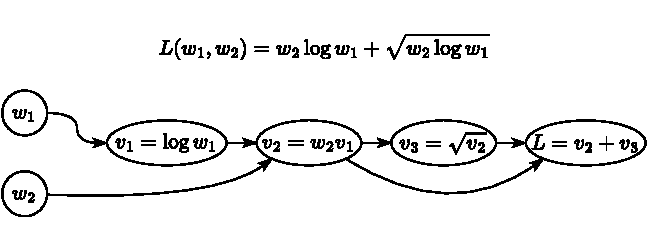
\includegraphics[keepaspectratio]{comp_graph.pdf}}

}

\caption{Иллюстрация вычислительного графа для функции \(L(w_1, w_2)\)}

\end{figure}%

Давайте пойдем от начала графа к концу и вычислим производную
\(\dfrac{\partial L}{\partial w_1}\).

\begin{figure}[H]

{\centering \pandocbounded{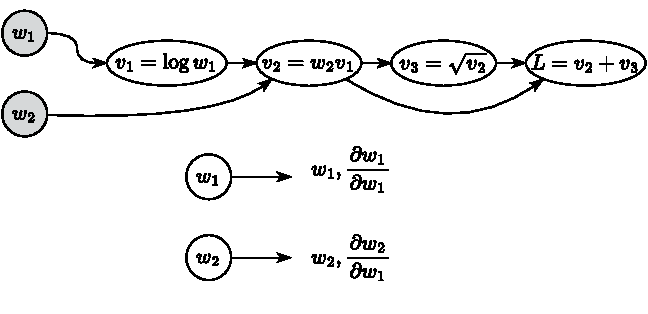
\includegraphics[keepaspectratio]{comp_graph1.pdf}}

}

\caption{Иллюстрация прямого режима автоматического дифференцирования}

\end{figure}%

\textbf{Функция}

\(w_1 = w_1, w_2 = w_2\)

\textbf{Производная}

\(\dfrac{\partial w_1}{\partial w_1} = 1, \dfrac{\partial w_2}{\partial w_1} = 0\)

\begin{figure}[H]

{\centering \pandocbounded{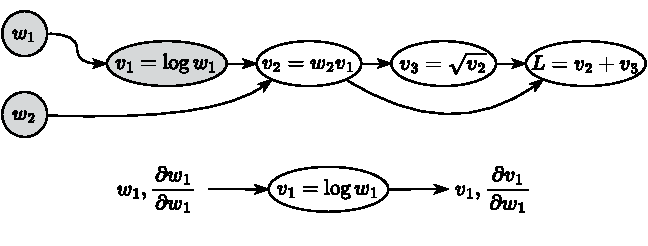
\includegraphics[keepaspectratio]{comp_graph2.pdf}}

}

\caption{Иллюстрация прямого режима автоматического дифференцирования}

\end{figure}%

\textbf{Функция}

\(v_1 = \log w_1\)

\textbf{Производная}

\(\frac{\partial v_1}{\partial w_1} = \frac{\partial v_1}{\partial w_1} \frac{\partial w_1}{\partial w_1} = \frac{1}{w_1} 1\)

\begin{figure}[H]

{\centering \pandocbounded{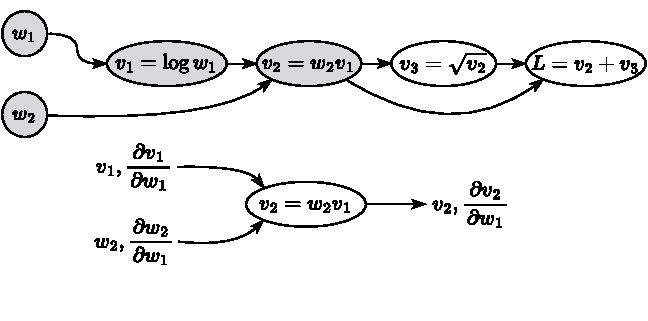
\includegraphics[keepaspectratio]{comp_graph3.pdf}}

}

\caption{Иллюстрация прямого режима автоматического дифференцирования}

\end{figure}%

\textbf{Функция}

\(v_2 = w_2 v_1\)

\textbf{Производная}

\(\frac{\partial v_2}{\partial w_1} = \frac{\partial v_2}{\partial v_1}\frac{\partial v_1}{\partial w_1} + \frac{\partial v_2}{\partial w_2}\frac{\partial w_2}{\partial w_1} = w_2\frac{\partial v_1}{\partial w_1} + v_1\frac{\partial w_2}{\partial w_1}\)

\begin{figure}[H]

{\centering \pandocbounded{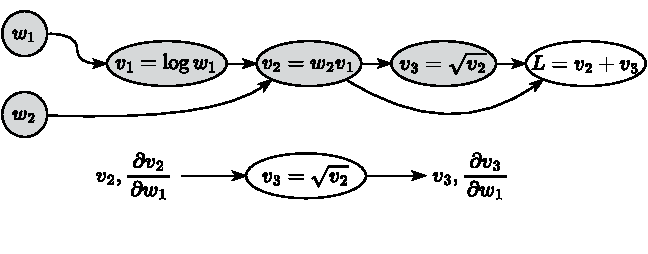
\includegraphics[keepaspectratio]{comp_graph4.pdf}}

}

\caption{Иллюстрация прямого режима автоматического дифференцирования}

\end{figure}%

\textbf{Функция}

\(v_3 = \sqrt{v_2}\)

\textbf{Производная}

\(\frac{\partial v_3}{\partial w_1} = \frac{\partial v_3}{\partial v_2}\frac{\partial v_2}{\partial w_1} = \frac{1}{2\sqrt{v_2}}\frac{\partial v_2}{\partial w_1}\)

\begin{figure}[H]

{\centering \pandocbounded{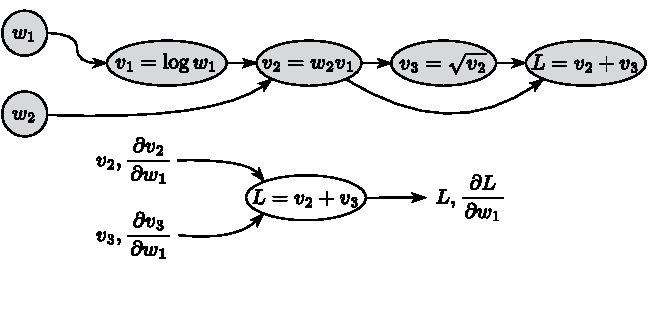
\includegraphics[keepaspectratio]{comp_graph5.pdf}}

}

\caption{Иллюстрация прямого режима автоматического дифференцирования}

\end{figure}%

\textbf{Функция}

\(L = v_2 + v_3\)

\textbf{Производная}

\(\frac{\partial L}{\partial w_1} = \frac{\partial L}{\partial v_2}\frac{\partial v_2}{\partial w_1} + \frac{\partial L}{\partial v_3}\frac{\partial v_3}{\partial w_1} = 1\frac{\partial v_2}{\partial w_1} + 1\frac{\partial v_3}{\partial w_1}\)

\textbf{Сделайте аналогичные вычисления для
\(\dfrac{\partial L}{\partial w_2}\)}

\begin{figure}[H]

{\centering \pandocbounded{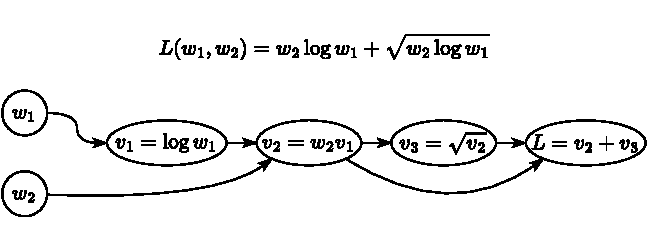
\includegraphics[keepaspectratio]{comp_graph.pdf}}

}

\caption{Иллюстрация вычислительного графа для функции \(L(w_1, w_2)\)}

\end{figure}%

\begin{figure}[H]

{\centering \pandocbounded{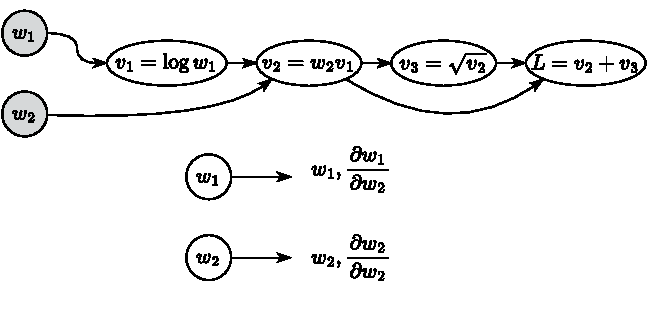
\includegraphics[keepaspectratio]{cgraph_ex_1.pdf}}

}

\caption{Иллюстрация прямого режима автоматического дифференцирования}

\end{figure}%

\textbf{Функция}

\(w_1 = w_1, w_2 = w_2\)

\textbf{Производная}

\(\dfrac{\partial w_1}{\partial w_2} = 0, \dfrac{\partial w_2}{\partial w_2} = 1\)

\begin{figure}[H]

{\centering \pandocbounded{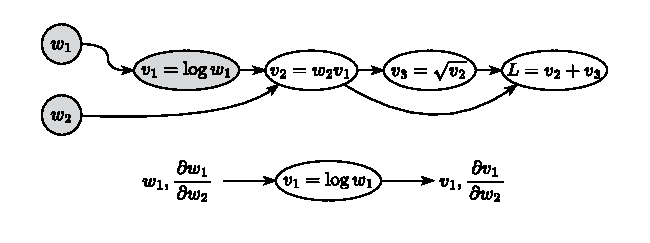
\includegraphics[keepaspectratio]{cgraph_ex_2.pdf}}

}

\caption{Иллюстрация прямого режима автоматического дифференцирования}

\end{figure}%

\textbf{Функция}

\(v_1 = \log w_1\)

\textbf{Производная}

\(\frac{\partial v_1}{\partial w_2} = \frac{\partial v_1}{\partial w_1} \frac{\partial w_1}{\partial w_2}= \frac{1}{w_1} \cdot 0\)

\begin{figure}[H]

{\centering \pandocbounded{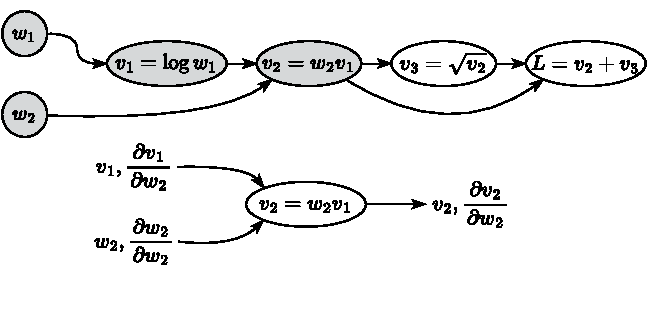
\includegraphics[keepaspectratio]{cgraph_ex_3.pdf}}

}

\caption{Иллюстрация прямого режима автоматического дифференцирования}

\end{figure}%

\textbf{Функция}

\(v_2 = w_2 v_1\)

\textbf{Производная}

\(\frac{\partial v_2}{\partial w_2} = \frac{\partial v_2}{\partial v_1}\frac{\partial v_1}{\partial w_2} + \frac{\partial v_2}{\partial w_2}\frac{\partial w_2}{\partial w_2} = w_2\frac{\partial v_1}{\partial w_2} + v_1\frac{\partial w_2}{\partial w_2}\)

\begin{figure}[H]

{\centering \pandocbounded{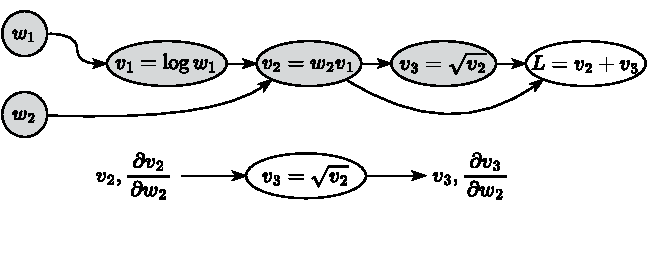
\includegraphics[keepaspectratio]{cgraph_ex_4.pdf}}

}

\caption{Иллюстрация прямого режима автоматического дифференцирования}

\end{figure}%

\textbf{Функция}

\(v_3 = \sqrt{v_2}\)

\textbf{Производная}

\(\frac{\partial v_3}{\partial w_2} = \frac{\partial v_3}{\partial v_2}\frac{\partial v_2}{\partial w_2} = \frac{1}{2\sqrt{v_2}}\frac{\partial v_2}{\partial w_2}\)

\begin{figure}[H]

{\centering \pandocbounded{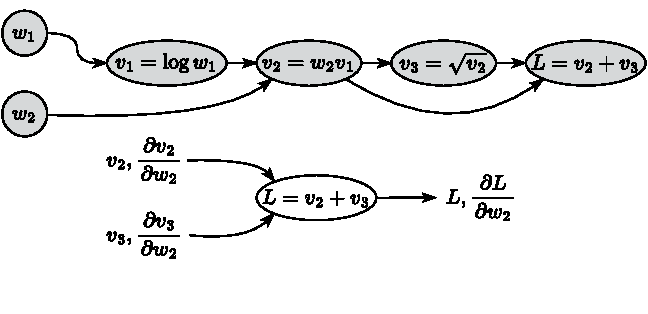
\includegraphics[keepaspectratio]{cgraph_ex_5.pdf}}

}

\caption{Иллюстрация прямого режима автоматического дифференцирования}

\end{figure}%

\textbf{Функция}

\(L = v_2 + v_3\)

\textbf{Производная}

\(\frac{\partial L}{\partial w_2} = \frac{\partial L}{\partial v_2}\frac{\partial v_2}{\partial w_2} + \frac{\partial L}{\partial v_3}\frac{\partial v_3}{\partial w_2} = 1\frac{\partial v_2}{\partial w_2} + 1\frac{\partial v_3}{\partial w_2}\)

\subsection{Алгоритм прямого режима автоматического
дифференцирования}\label{ux430ux43bux433ux43eux440ux438ux442ux43c-ux43fux440ux44fux43cux43eux433ux43e-ux440ux435ux436ux438ux43cux430-ux430ux432ux442ux43eux43cux430ux442ux438ux447ux435ux441ux43aux43eux433ux43e-ux434ux438ux444ux444ux435ux440ux435ux43dux446ux438ux440ux43eux432ux430ux43dux438ux44f}

Предположим, что у нас есть вычислительный граф \(v_i, i \in [1; N]\).
Наша цель - вычислить производную выхода этого графа по некоторой
входной переменной \(w_k\), т.е. \(\dfrac{\partial v_N}{\partial w_k}\).
Эта идея предполагает распространение градиента по входной переменной от
начала к концу, поэтому мы можем ввести обозначение:

\[
\overline{v_i} = \dfrac{\partial v_i}{\partial w_k}
\]
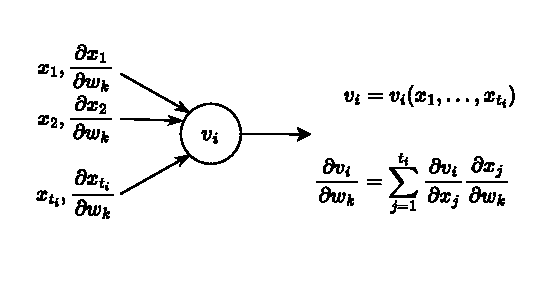
\includegraphics[width=0.6\linewidth,height=\textheight,keepaspectratio]{auto_diff_forward.pdf}

\begin{itemize}
\tightlist
\item
  Для \(i = 1, \ldots, N\):

  \begin{itemize}
  \tightlist
  \item
    Вычислить \(v_i\) как функцию его предков \(x_1, \ldots, x_{t_i}\):
    \[
      v_i = v_i(x_1, \ldots, x_{t_i})
      \]
  \item
    Вычислить производную \(\overline{v_i}\) используя формулу
    производной сложной функции: \[
      \overline{v_i} = \sum_{j = 1}^{t_i}\dfrac{\partial v_i}{\partial x_j}\dfrac{\partial x_j}{\partial w_k}
      \]
  \end{itemize}
\end{itemize}

Обратите внимание, что этот подход не требует хранения всех
промежуточных вычислений, но можно видеть, что для вычисления
производной \(\dfrac{\partial L}{\partial w_k}\) нам нужно
\(\mathcal{O}(T)\) операций. Это означает, что для всего градиента, нам
нужно \(d\mathcal{O}(T)\) операций, что то же самое, что и для конечных
разностей, но теперь у нас нет проблем со стабильностью или
неточностями(формулы выше точны).

\pandocbounded{
\includegraphics[keepaspectratio]{yoda.jpg}}

\subsection{Обратный режим автоматического
дифференцирования}\label{ux43eux431ux440ux430ux442ux43dux44bux439-ux440ux435ux436ux438ux43c-ux430ux432ux442ux43eux43cux430ux442ux438ux447ux435ux441ux43aux43eux433ux43e-ux434ux438ux444ux444ux435ux440ux435ux43dux446ux438ux440ux43eux432ux430ux43dux438ux44f}

Мы рассмотрим ту же функцию с вычислительным графом:

\begin{figure}[H]

{\centering \pandocbounded{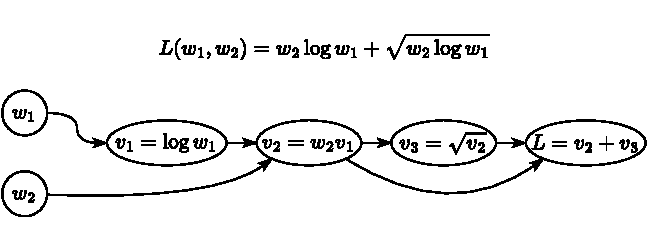
\includegraphics[keepaspectratio]{comp_graph.pdf}}

}

\caption{Иллюстрация вычислительного графа для функции \(L(w_1, w_2)\)}

\end{figure}%

Предположим, что у нас есть некоторые значения параметров \(w_1, w_2\) и
мы уже выполнили прямой проход (т.е. вычисление значений всех
промежуточных узлов вычислительного графа). Предположим также, что мы
как-то сохранили все промежуточные значения \(v_i\). Давайте пойдем от
конца графа к началу и вычислим производные
\(\dfrac{\partial L}{\partial w_1}, \dfrac{\partial L}{\partial w_2}\):

\begin{figure}[H]

{\centering \pandocbounded{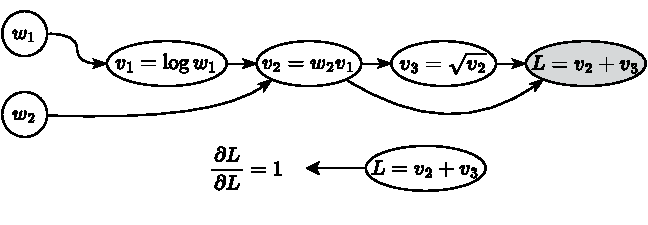
\includegraphics[keepaspectratio]{revad1.pdf}}

}

\caption{Иллюстрация обратного режима автоматического дифференцирования}

\end{figure}%

\textbf{Производные}

\[
\dfrac{\partial L}{\partial L} = 1
\]

\begin{figure}[H]

{\centering \pandocbounded{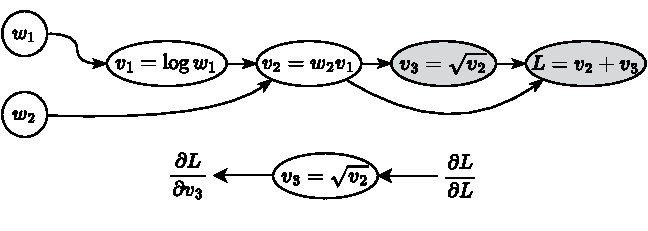
\includegraphics[keepaspectratio]{revad2.pdf}}

}

\caption{Иллюстрация обратного режима автоматического дифференцирования}

\end{figure}%

\textbf{Производные}

\[
\begin{aligned}\frac{\partial L}{\partial v_3} &= \frac{\partial L}{\partial L} \frac{\partial L}{\partial v_3} &= \frac{\partial L}{\partial L} 1\end{aligned}
\]

\begin{figure}[H]

{\centering \pandocbounded{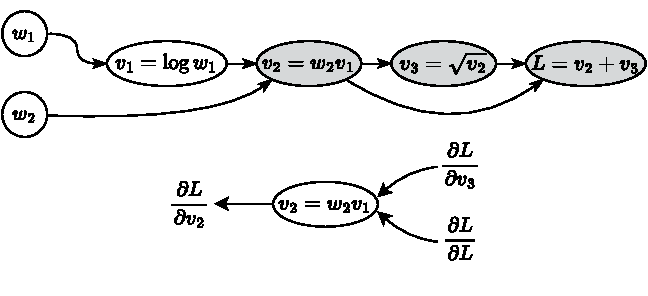
\includegraphics[keepaspectratio]{revad3.pdf}}

}

\caption{Иллюстрация обратного режима автоматического дифференцирования}

\end{figure}%

\textbf{Производные}

\[
\begin{aligned}\frac{\partial L}{\partial v_2} &= \frac{\partial L}{\partial v_3}\frac{\partial v_3}{\partial v_2} + \frac{\partial L}{\partial L}\frac{\partial L}{\partial v_2} &= \frac{\partial L}{\partial v_3}\frac{1}{2\sqrt{v_2}} +  \frac{\partial L}{\partial L}1\end{aligned}
\]

\begin{figure}[H]

{\centering \pandocbounded{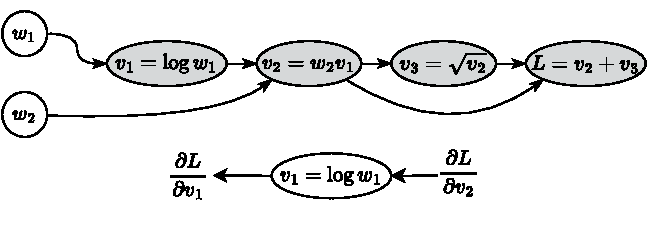
\includegraphics[keepaspectratio]{revad4.pdf}}

}

\caption{Иллюстрация обратного режима автоматического дифференцирования}

\end{figure}%

\textbf{Производные}

\[
\begin{aligned}\frac{\partial L}{\partial v_1} &=\frac{\partial L}{\partial v_2}\frac{\partial v_2}{\partial v_1}  &= \frac{\partial L}{\partial v_2}w_2\end{aligned}
\]

\begin{figure}[H]

{\centering \pandocbounded{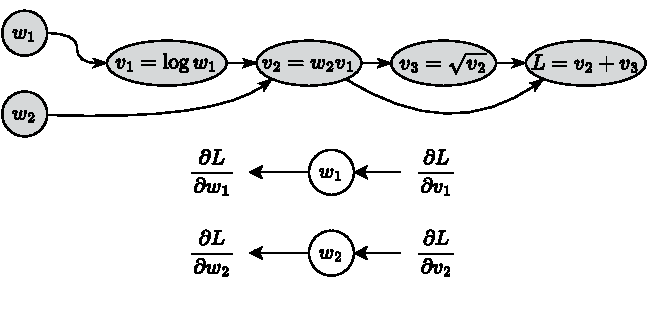
\includegraphics[keepaspectratio]{revad5.pdf}}

}

\caption{Иллюстрация обратного режима автоматического дифференцирования}

\end{figure}%

\textbf{Производные}

\[
\frac{\partial L}{\partial w_1} = \frac{\partial L}{\partial v_1}\frac{\partial v_1}{\partial w_1} = \frac{\partial L}{\partial v_1}\frac{1}{w_1} \qquad \qquad \frac{\partial L}{\partial w_2} = \frac{\partial L}{\partial v_2}\frac{\partial v_2}{\partial w_2} = \frac{\partial L}{\partial v_1}v_1
\]

\subsection{Обратный режим автоматического
дифференцирования}\label{ux43eux431ux440ux430ux442ux43dux44bux439-ux440ux435ux436ux438ux43c-ux430ux432ux442ux43eux43cux430ux442ux438ux447ux435ux441ux43aux43eux433ux43e-ux434ux438ux444ux444ux435ux440ux435ux43dux446ux438ux440ux43eux432ux430ux43dux438ux44f-1}

\begin{tcolorbox}[enhanced jigsaw, colframe=quarto-callout-color-frame, rightrule=.15mm, toprule=.15mm, coltitle=black, opacityback=0, colback=white, leftrule=.75mm, arc=.35mm, opacitybacktitle=0.6, bottomrule=.15mm, breakable, toptitle=1mm, colbacktitle=quarto-callout-color!10!white, bottomtitle=1mm, title=\textcolor{quarto-callout-color}{\faInfo}\hspace{0.5em}{Question}, left=2mm, titlerule=0mm]

Обратите внимание, что для того же количества вычислений, что и в прямом
режиме, мы получаем полный вектор градиента \(\nabla_w L\). Какова
стоимость ускорения?

\textbf{Ответ} Обратите внимание, что для использования обратного режима
AD вам нужно хранить все промежуточные вычисления из прямого прохода.
Эта проблема может быть частично решена с помощью чекпоинтинга, при
котором мы сохраняем только часть промежуточных значений, а остальные
пересчитываем заново по мере необходимости. Это позволяет значительно
уменьшить объём требуемой памяти при обучении больших моделей машинного
обучения.

\end{tcolorbox}

\subsection{Алгоритм обратного режима автоматического
дифференцирования}\label{ux430ux43bux433ux43eux440ux438ux442ux43c-ux43eux431ux440ux430ux442ux43dux43eux433ux43e-ux440ux435ux436ux438ux43cux430-ux430ux432ux442ux43eux43cux430ux442ux438ux447ux435ux441ux43aux43eux433ux43e-ux434ux438ux444ux444ux435ux440ux435ux43dux446ux438ux440ux43eux432ux430ux43dux438ux44f}

Предположим, что у нас есть вычислительный граф \(v_i, i \in [1; N]\).
Наша цель - вычислить производную выхода этого графа по всем входным
переменным \(w\), т.е.
\(\nabla_w v_N =  \left( \frac{\partial v_N}{\partial w_1}, \ldots, \frac{\partial v_N}{\partial w_d}\right)^T\).
Эта идея предполагает распространение градиента функции по промежуточным
переменным от конца к началу, поэтому мы можем ввести обозначение: \[
\overline{v_i}  = \dfrac{\partial L}{\partial v_i} = \dfrac{\partial v_N}{\partial v_i}
\]
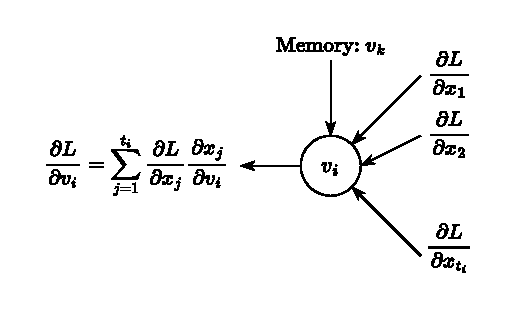
\includegraphics[width=0.6\linewidth,height=\textheight,keepaspectratio]{auto_diff_reverse.pdf}

\begin{itemize}
\item
  \textbf{ПРЯМОЙ ПРОХОД}

  Для \(i = 1, \ldots, N\):

  \begin{itemize}
  \tightlist
  \item
    Вычислить и сохранить значения \(v_i\) как функцию его предков
  \end{itemize}
\item
  \textbf{ОБРАТНЫЙ ПРОХОД}

  Для \(i = N, \ldots, 1\):

  \begin{itemize}
  \tightlist
  \item
    Вычислить производную \(\overline{v_i}\) используя формулу
    производной сложной функции и информацию от всех потомков (выходов):
    \[
      \overline{v_i} = \dfrac{\partial L}{\partial v_i} = \sum_{j = 1}^{t_i} \dfrac{\partial L}{\partial x_j} \dfrac{\partial x_j}{\partial v_i}
      \]
  \end{itemize}
\end{itemize}

\newpage

\textbf{Choose your fighter}

\begin{figure}[H]

{\centering \pandocbounded{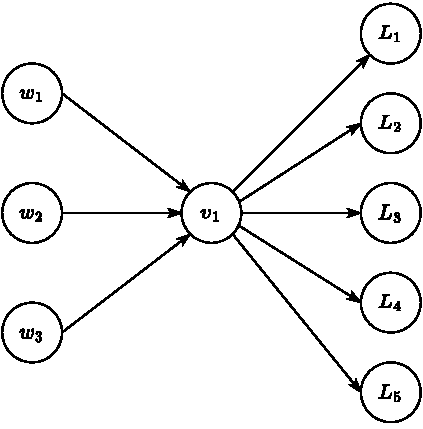
\includegraphics[keepaspectratio]{ad_choose.pdf}}

}

\caption{Какой режим вы бы выбрали для вычисления градиентов?}

\end{figure}%

\begin{tcolorbox}[enhanced jigsaw, colframe=quarto-callout-color-frame, rightrule=.15mm, toprule=.15mm, coltitle=black, opacityback=0, colback=white, leftrule=.75mm, arc=.35mm, opacitybacktitle=0.6, bottomrule=.15mm, breakable, toptitle=1mm, colbacktitle=quarto-callout-color!10!white, bottomtitle=1mm, title=\textcolor{quarto-callout-color}{\faInfo}\hspace{0.5em}{Question}, left=2mm, titlerule=0mm]

Какой из режимов AD вы бы выбрали (прямой/обратный) для следующего
вычислительного графа арифметических операций? Предположим, что вам
нужно вычислить якобиан
\(J = \left\{ \dfrac{\partial L_i}{\partial w_j} \right\}_{i,j}\)

\end{tcolorbox}

\textbf{Ответ} Обратите внимание, что время вычислений в обратном режиме
пропорционально количеству выходов, тогда как время работы прямого
режима пропорционально количеству входов. Поэтому было бы хорошей идеей
рассмотреть прямой режим AD.

\begin{figure}[H]

{\centering 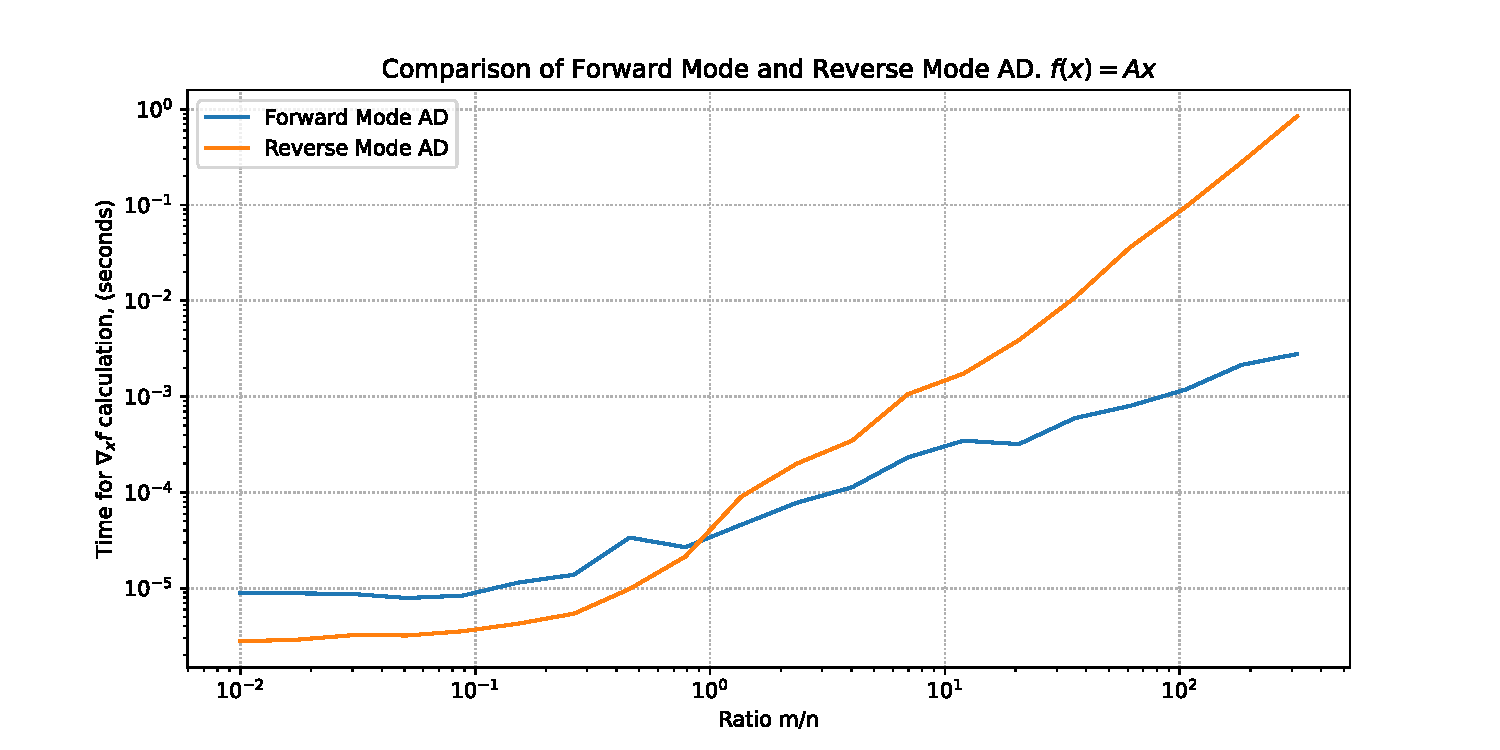
\includegraphics[width=0.88\linewidth,height=\textheight,keepaspectratio]{forward_vs_reverse_ad.pdf}

}

\caption{\href{https://colab.research.google.com/github/MerkulovDaniil/optim/blob/master/assets/Notebooks/Autograd_and_Jax.ipynb}{\(\clubsuit\)}
График иллюстрирует идею выбора между режимами автоматического
дифференцирования. Размерность входа \(n = 100\) фиксирована, измерено
время вычисления якобиана в зависимости от соотношения размерностей
выхода и входа для разных размерностей выхода \(m\).}

\end{figure}%

\textbf{Choose your fighter}

\begin{figure}[H]

{\centering \pandocbounded{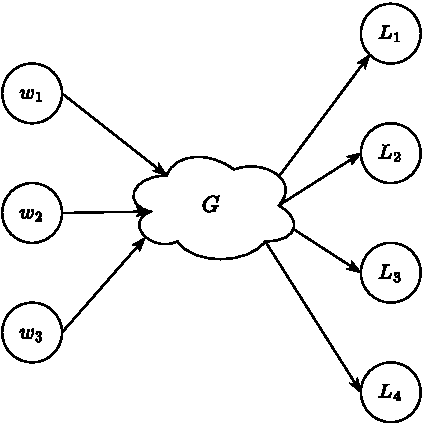
\includegraphics[keepaspectratio]{ad_mixed.pdf}}

}

\caption{Какой режим вы бы выбрали для вычисления градиентов?}

\end{figure}%

\begin{tcolorbox}[enhanced jigsaw, colframe=quarto-callout-color-frame, rightrule=.15mm, toprule=.15mm, coltitle=black, opacityback=0, colback=white, leftrule=.75mm, arc=.35mm, opacitybacktitle=0.6, bottomrule=.15mm, breakable, toptitle=1mm, colbacktitle=quarto-callout-color!10!white, bottomtitle=1mm, title=\textcolor{quarto-callout-color}{\faInfo}\hspace{0.5em}{Question}, left=2mm, titlerule=0mm]

Какой из режимов AD вы бы выбрали (прямой/обратный) для следующего
вычислительного графа арифметических операций? Предположим, что вам
нужно вычислить якобиан
\(J = \left\{ \dfrac{\partial L_i}{\partial w_j} \right\}_{i,j}\).
Обратите внимание, что \(G\) - это произвольный вычислительный граф

\end{tcolorbox}

\textbf{Ответ} В общем случае невозможно ответить без некоторого знания
о конкретной структуре графа \(G\). Следует отметить, что существуют
продвинутые подходы, смешивающие прямой и обратный режим AD в
зависимости от конкретной структуры графа \(G\).

\subsection{Архитектура прямого
распространения}\label{ux430ux440ux445ux438ux442ux435ux43aux442ux443ux440ux430-ux43fux440ux44fux43cux43eux433ux43e-ux440ux430ux441ux43fux440ux43eux441ux442ux440ux430ux43dux435ux43dux438ux44f}

\textbf{ПРЯМОЙ ПРОХОД}

\begin{itemize}
\item
  \(v_0 = x\) на вход обычно подаётся батч данных \(x\)
\item
  Для \(k = 1, \ldots, t-1, t\):

  \begin{itemize}
  \tightlist
  \item
    \(v_k = \sigma(v_{k-1}w_k)\). Обратите внимание, что на практике,
    данные имеют размерность \(x  \in \mathbb{R}^{b \times d}\), где
    \(b\) - размер батча (для одного объекта из выборки \(b=1\)). В то
    время как матрица весов \(w_k\) \(k\) слоя имеет размер
    \(n_{k-1} \times n_k\), где \(n_k\) - размер внутреннего
    представления данных.
  \end{itemize}
\item
  \(L = L(v_t)\) - вычислить функцию потерь.
\end{itemize}

\textbf{ОБРАТНЫЙ ПРОХОД}

\begin{itemize}
\item
  \(v_{t+1} = L, \dfrac{\partial L}{\partial L} = 1\)
\item
  Для \(k = t, t-1, \ldots, 1\):

  \begin{itemize}
  \tightlist
  \item
    \(\underset{b \times n_k}{\dfrac{\partial L}{\partial v_k}} = \underset{b \times n_{k+1}}{\dfrac{\partial L}{\partial v_{k+1}}} \underset{n_{k+1} \times n_k}{\dfrac{\partial v_{k+1}}{\partial v_{k}}}\)
  \item
    \(\underset{b \times n_{k-1} \cdot n_k}{\dfrac{\partial L}{\partial w_k}} = \underset{b \times n_{k+1}}{\dfrac{\partial L}{\partial v_{k+1}}} \cdot  \underset{n_{k+1} \times n_{k-1} \cdot n_k}{\dfrac{\partial v_{k+1}}{\partial w_{k}}}\)
  \end{itemize}
\end{itemize}

\begin{figure}[H]

{\centering \pandocbounded{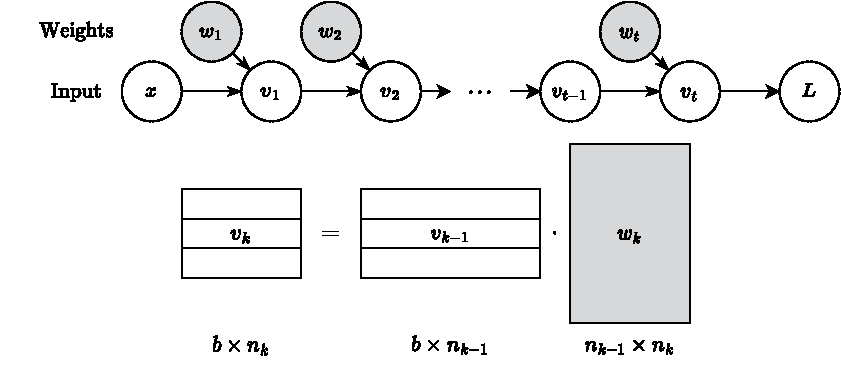
\includegraphics[keepaspectratio]{feedforward.pdf}}

}

\caption{Архитектура прямого распространения нейронной сети}

\end{figure}%

\subsection{Произведение Гессиана на вектор без вычисления самого
Гессиана}\label{ux43fux440ux43eux438ux437ux432ux435ux434ux435ux43dux438ux435-ux433ux435ux441ux441ux438ux430ux43dux430-ux43dux430-ux432ux435ux43aux442ux43eux440-ux431ux435ux437-ux432ux44bux447ux438ux441ux43bux435ux43dux438ux44f-ux441ux430ux43cux43eux433ux43e-ux433ux435ux441ux441ux438ux430ux43dux430}

Когда вам нужна некоторая информация о кривизне функции, обычно вам
нужно работать с гессианом. Однако, это трудно делать, когда размерность
задачи велика. Для скалярной функции
\(f : \mathbb{R}^n \to \mathbb{R}\), гессиан в точке
\(x \in \mathbb{R}^n\) записывается как \(\nabla^2 f(x)\). Тогда
произведение вектора на гессиан можно записать как

\[
v \mapsto \nabla^2 f(x) \cdot v
\]

для любого вектора \(v \in \mathbb{R}^n\). Мы можем использовать
тождество \[
\nabla^2 f (x) v = \nabla [x \mapsto \nabla f(x)^T \cdot v] = \nabla g(x),
\] где \(g(x) = \nabla f(x)^T \cdot v\) - новая функция, которая
скалярно умножает градиент \(f\) в \(x\) на вектор \(v\).

\begin{Shaded}
\begin{Highlighting}[]
\ImportTok{import}\NormalTok{ jax.numpy }\ImportTok{as}\NormalTok{ jnp}

\KeywordTok{def}\NormalTok{ hvp(f, x, v):}
    \ControlFlowTok{return}\NormalTok{ grad(}\KeywordTok{lambda}\NormalTok{ x: jnp.vdot(grad(f)(x), v))(x)}
\end{Highlighting}
\end{Shaded}

\subsection[Динамика обучения нейронной сети через спектр Гессиана и hvp
]{\texorpdfstring{Динамика обучения нейронной сети через спектр Гессиана
и hvp
\footnote{\href{https://arxiv.org/abs/1901.10159}{Некоторые исследования
  в оптимизации нейронных сетей через спектр собственных значений
  Гессиана}}}{Динамика обучения нейронной сети через спектр Гессиана и hvp }}\label{ux434ux438ux43dux430ux43cux438ux43aux430-ux43eux431ux443ux447ux435ux43dux438ux44f-ux43dux435ux439ux440ux43eux43dux43dux43eux439-ux441ux435ux442ux438-ux447ux435ux440ux435ux437-ux441ux43fux435ux43aux442ux440-ux433ux435ux441ux441ux438ux430ux43dux430-ux438-hvp}

\begin{figure}[H]

{\centering \pandocbounded{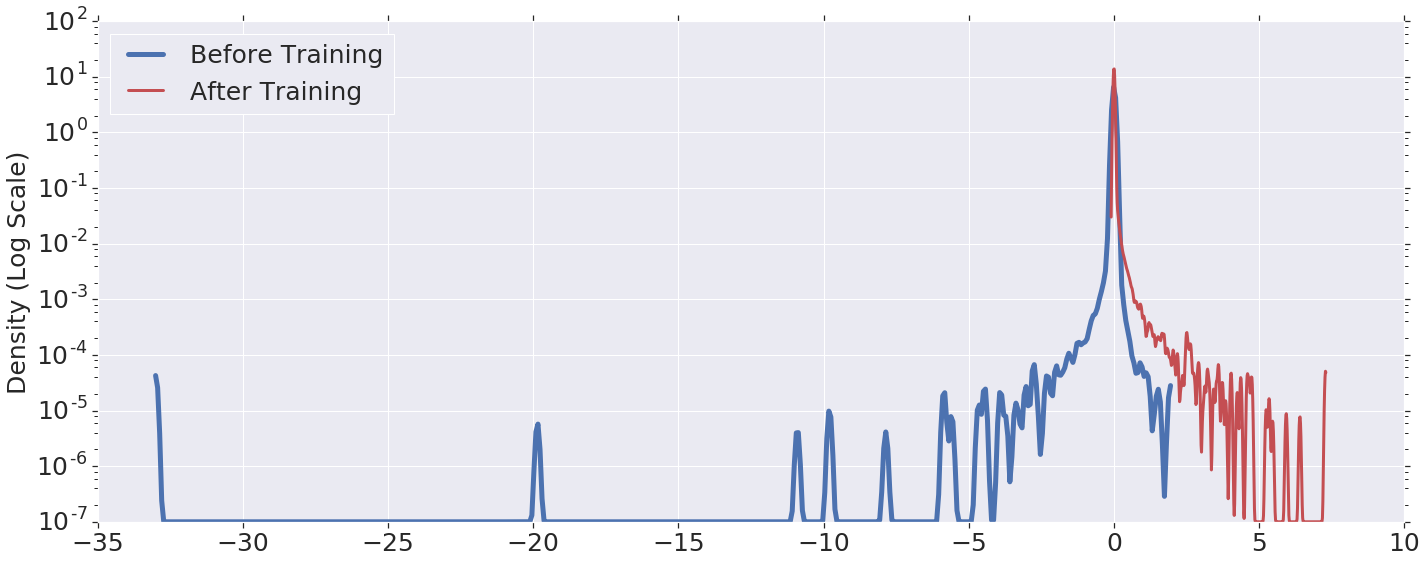
\includegraphics[keepaspectratio]{ResNet_32_before_After.png}}

}

\caption{Большие по модулю отрицательные собственные значения гессиана
исчезли после обучения ResNet-32}

\end{figure}%

\subsection[Идея Хадчинсона для оценки следа матрицы
]{\texorpdfstring{Идея Хадчинсона для оценки следа матрицы
\footnote{\href{https://www.tandfonline.com/doi/abs/10.1080/03610919008812866}{A
  stochastic estimator of the trace of the influence matrix for
  Laplacian smoothing splines - M.F. Hutchinson, 1990}}}{Идея Хадчинсона для оценки следа матрицы }}\label{ux438ux434ux435ux44f-ux445ux430ux434ux447ux438ux43dux441ux43eux43dux430-ux434ux43bux44f-ux43eux446ux435ux43dux43aux438-ux441ux43bux435ux434ux430-ux43cux430ux442ux440ux438ux446ux44b}

Метод Хатчинсона позволяет оценить след гессиана с помощью операций
вычисления умножения гессиана на произвольный вектор:

Пусть \(X \in \mathbb{R}^{d \times d}\) и \(v \in \mathbb{R}^d\) -
случайный вектор такой, что \(\mathbb{E}[vv^T] = I\). Тогда,

\[
\mathrm{Tr}(X) = \mathbb{E}[v^TXv] = \frac{1}{V}\sum_{i=1}^{V}v_i^TXv_i.
\]

\begin{figure}[H]

{\centering 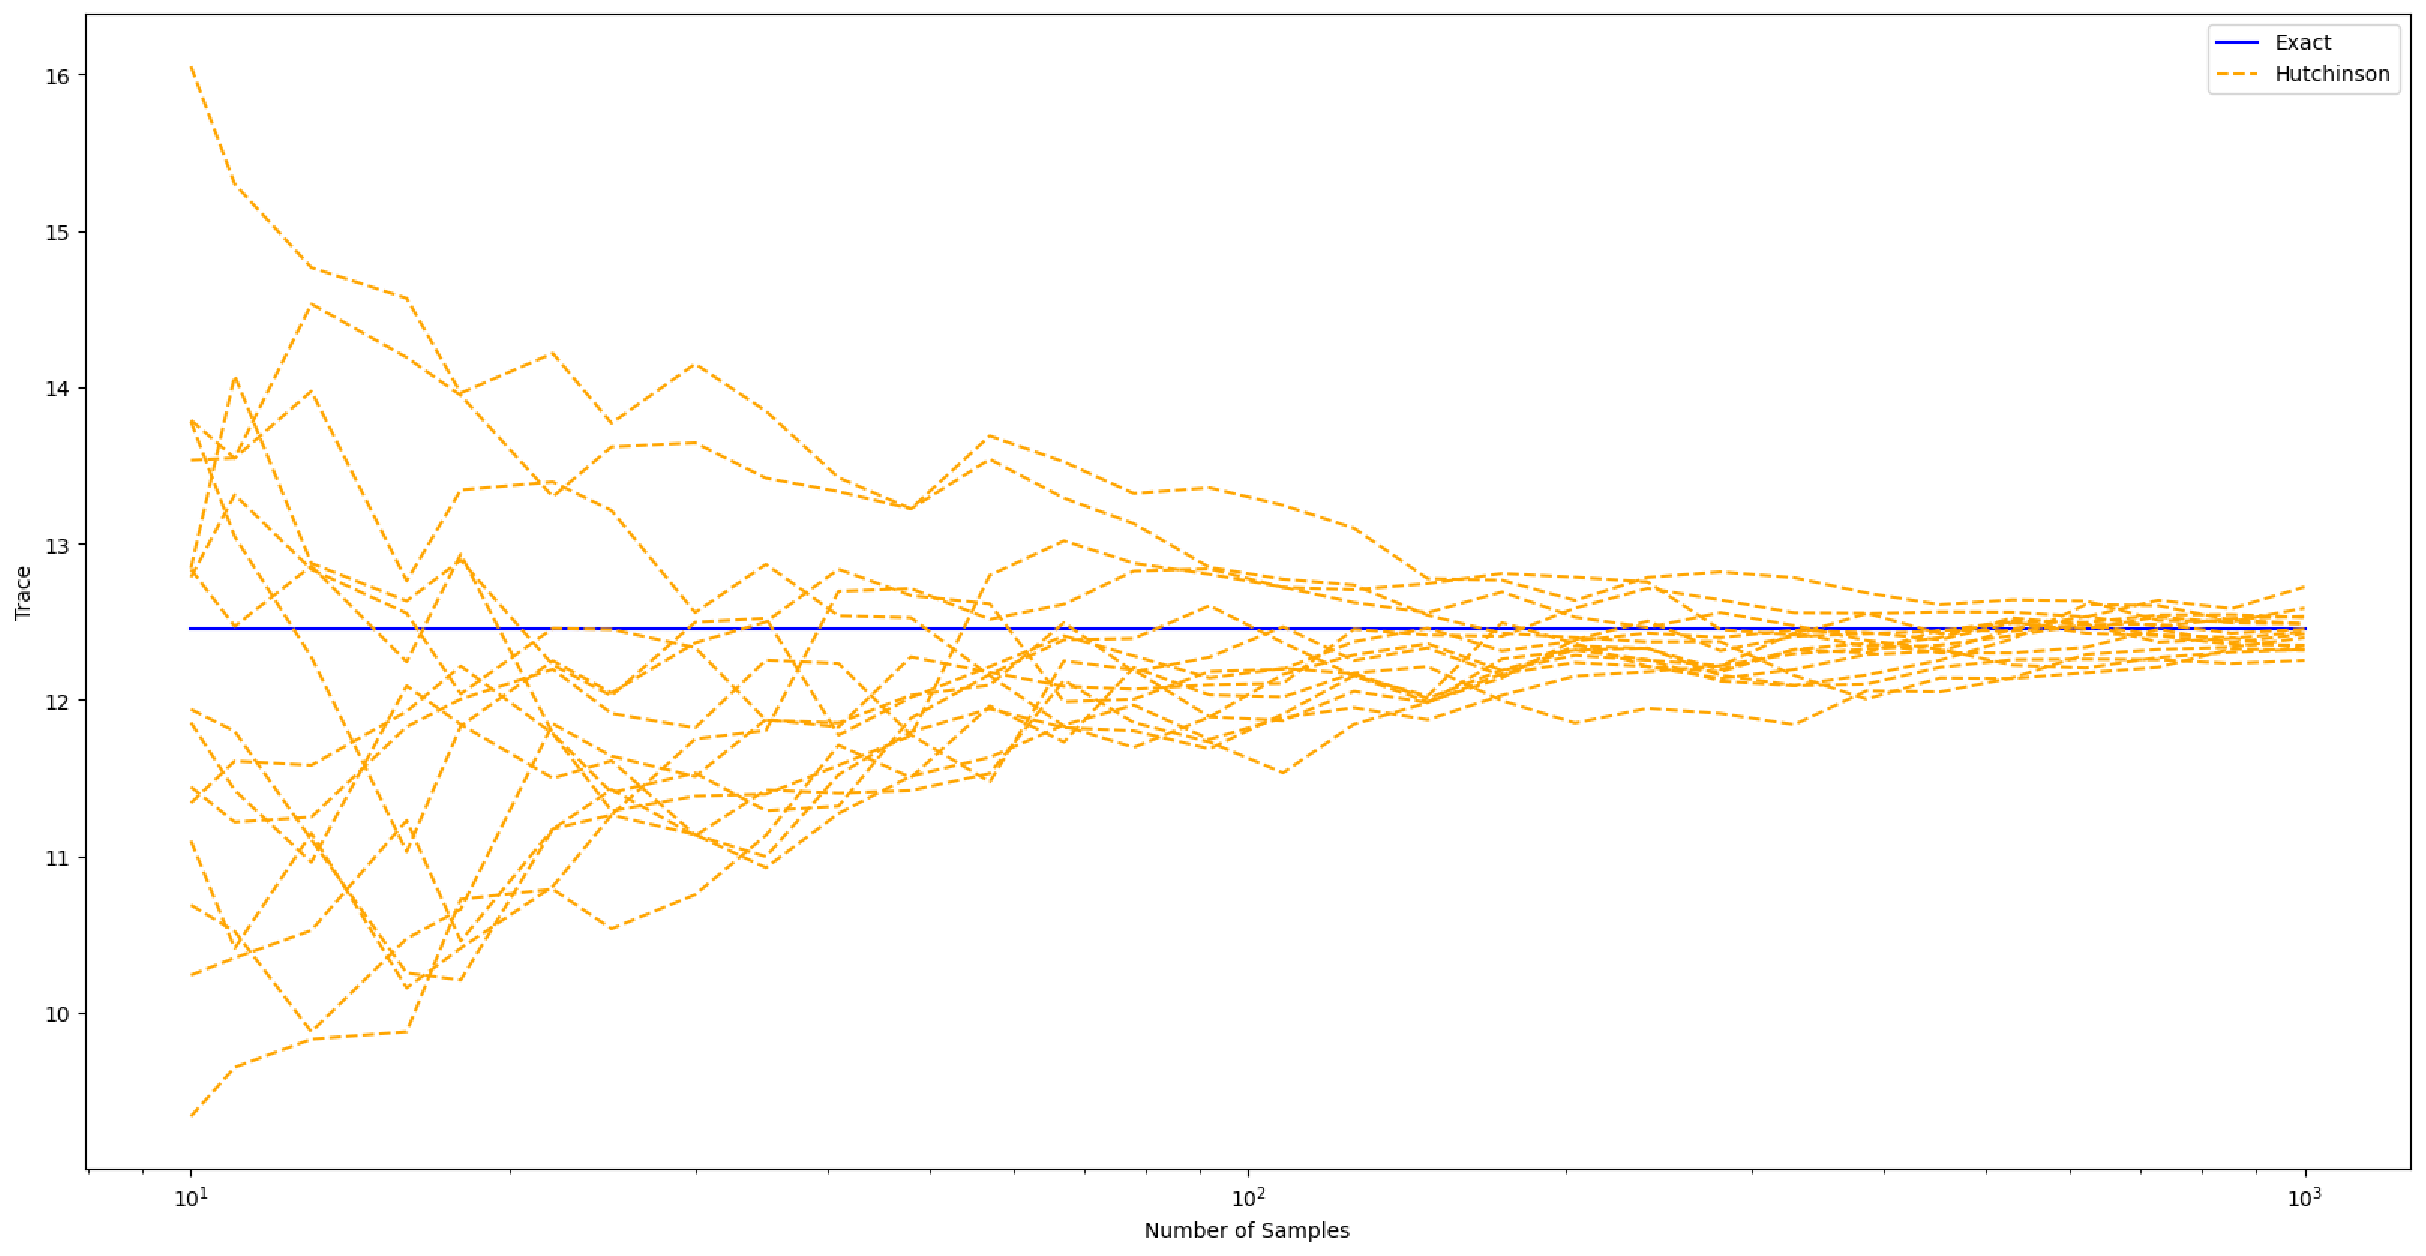
\includegraphics[width=0.8\linewidth,height=\textheight,keepaspectratio]{Hutchinson_trace_est.pdf}

}

\caption{\href{https://docs.backpack.pt/en/master/use_cases/example_trace_estimation.html}{Источник}}

\end{figure}%

\subsection{Чекпоинтинг}\label{ux447ux435ux43aux43fux43eux438ux43dux442ux438ux43dux433}

Анимация вышеуказанных подходов
\href{https://github.com/cybertronai/gradient-checkpointing}{\faGithub}

Пример использования контрольных точек градиента
\href{https://colab.research.google.com/github/oseledets/dl2023/blob/main/seminars/seminar-10/Large_model_training_practice.ipynb}{\faGithub}

В качестве примера рассмотрим обучение \textbf{GPT-2}\footnote{\href{https://arxiv.org/abs/1910.02054}{ZeRO:
  Memory Optimizations Toward Training Trillion Parameter Models}}:

\begin{itemize}
\tightlist
\item
  Активации в простом режиме могут занимать гораздо больше памяти: для
  последовательности длиной 1K и размера батча \(32\), \(60\) GB нужно
  для хранения всех промежуточных активаций.
\item
  Чекпоинтинг может снизить потребление до 8 GB, пересчитывая их (33\%
  дополнительных вычислений)
\end{itemize}

\subsection{Чем автоматическое дифференцирование (AD) не
является:}\label{ux447ux435ux43c-ux430ux432ux442ux43eux43cux430ux442ux438ux447ux435ux441ux43aux43eux435-ux434ux438ux444ux444ux435ux440ux435ux43dux446ux438ux440ux43eux432ux430ux43dux438ux435-ad-ux43dux435-ux44fux432ux43bux44fux435ux442ux441ux44f}

\begin{itemize}
\tightlist
\item
  AD не является методом конечных разностей
\item
  AD не является символьным вычислением производных
\item
  AD не является только правилом вычисления производной сложной функции
\item
  AD (обратный режим) является времяэффективным и численно стабильным
\item
  AD (обратный режим) не является эффективным по памяти (нужно хранить
  все промежуточные вычисления из прямого прохода)
\end{itemize}

\begin{figure}[H]

{\centering \pandocbounded{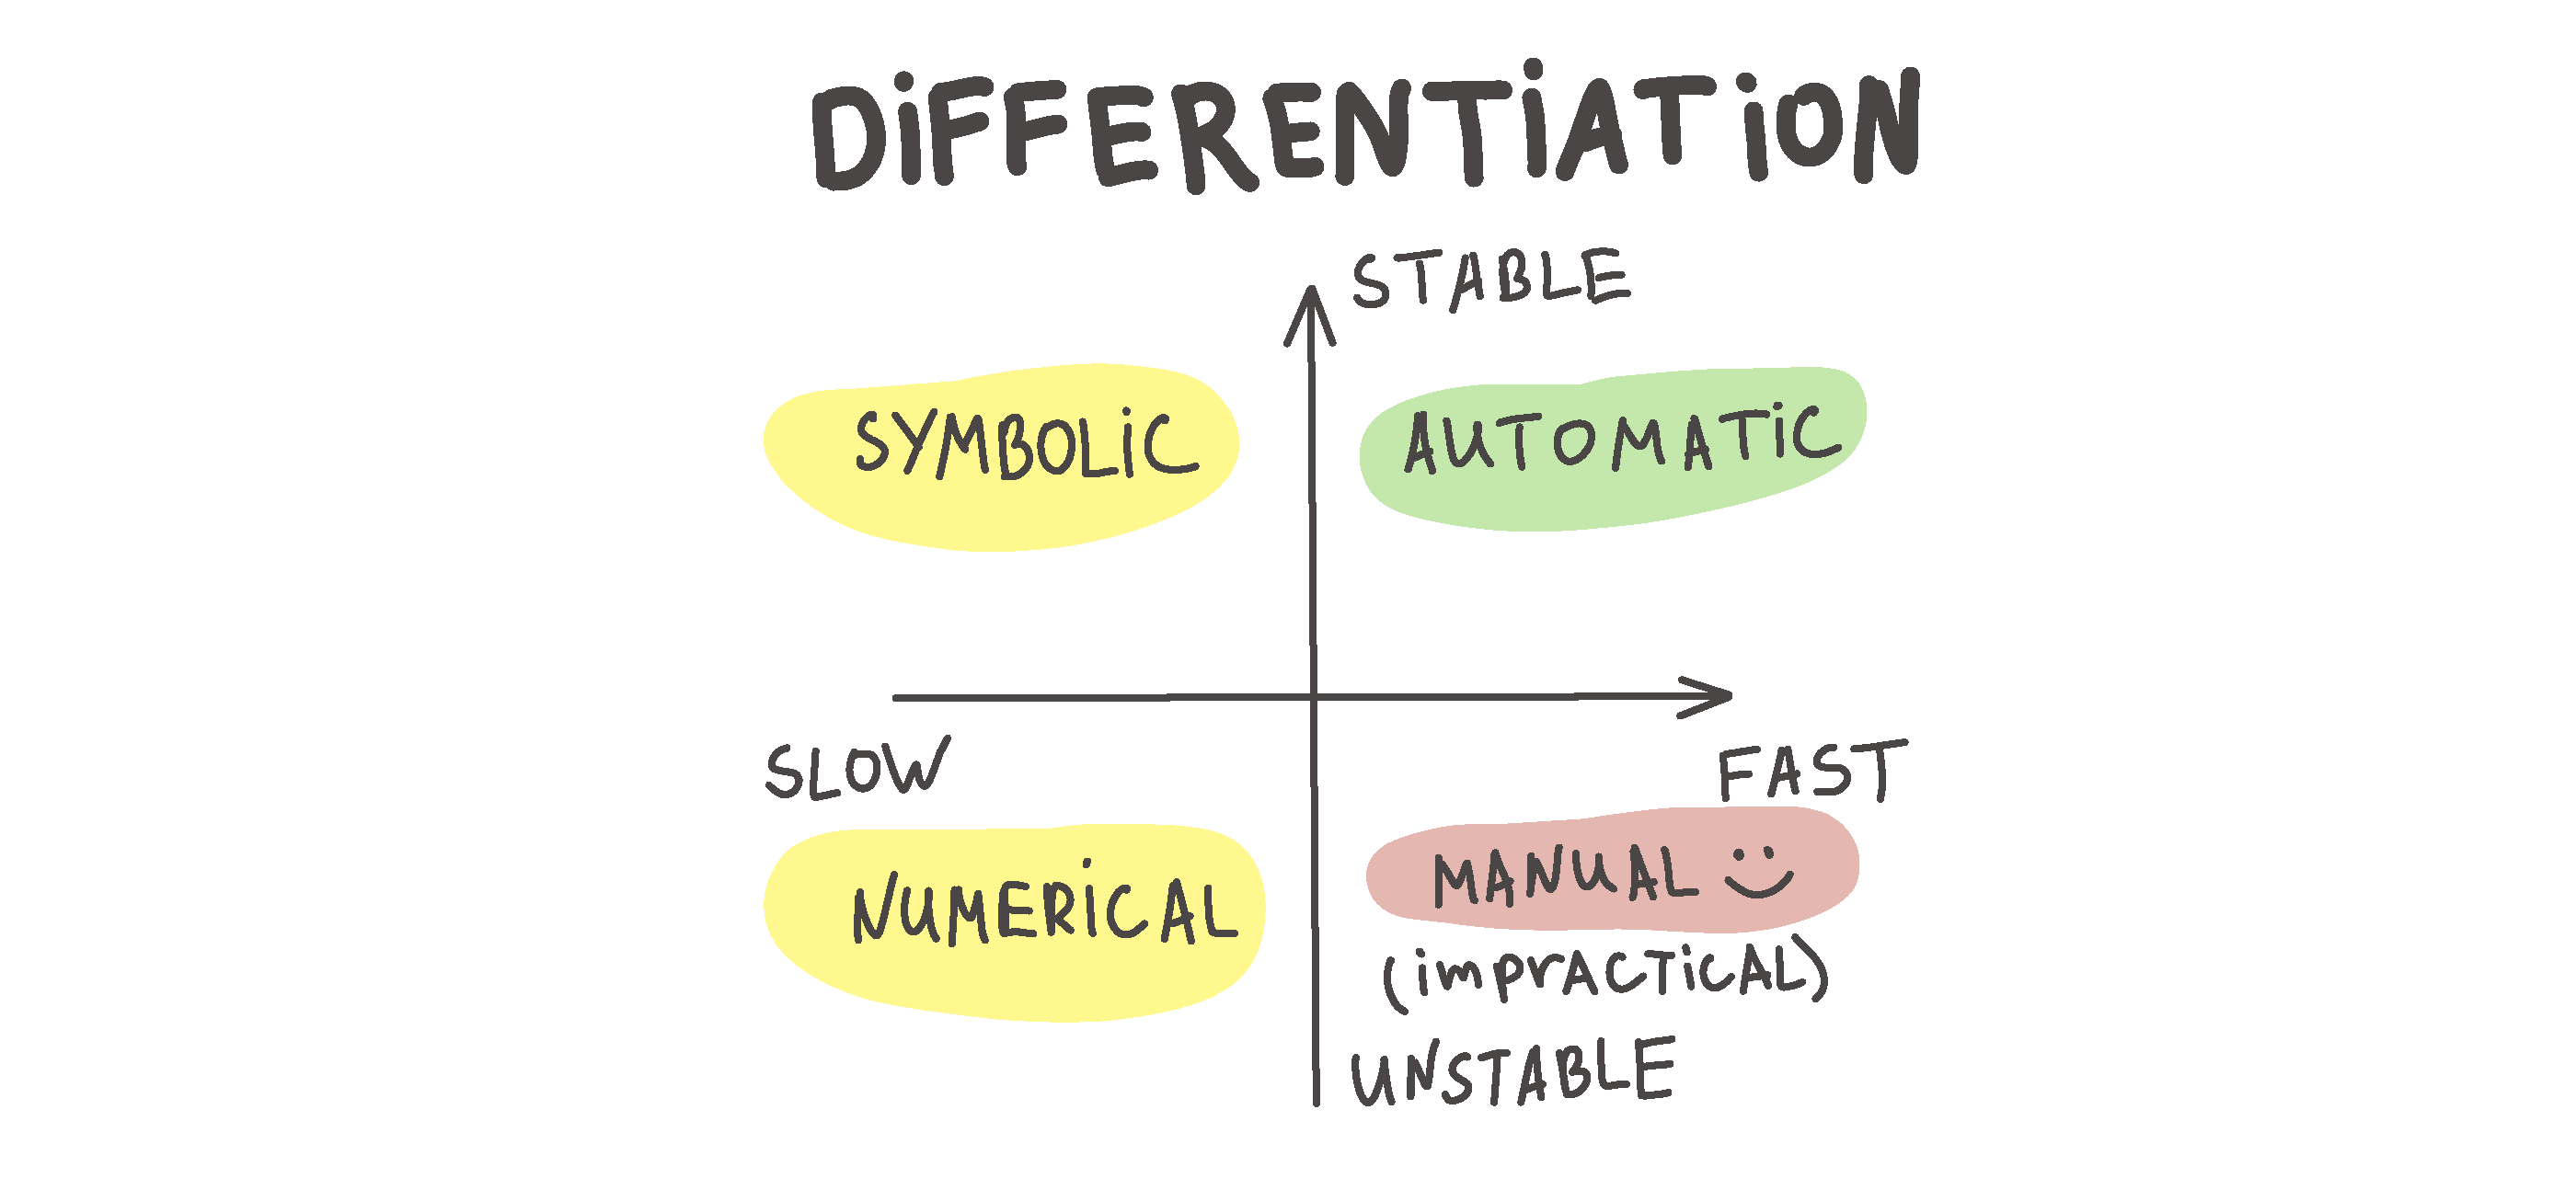
\includegraphics[keepaspectratio]{differentiation_scheme.pdf}}

}

\caption{Различные подходы для взятия производных}

\end{figure}%

\subsection{Дополнительные
материалы}\label{ux434ux43eux43fux43eux43bux43dux438ux442ux435ux43bux44cux43dux44bux435-ux43cux430ux442ux435ux440ux438ux430ux43bux44b}

\begin{itemize}
\tightlist
\item
  Рекомендую прочитать официальную книгу по Jax Autodiff.
  \href{https://colab.research.google.com/github/MerkulovDaniil/optim/blob/master/assets/Notebooks/Autograd_and_Jax.ipynb}{Open
  In Colab \(\clubsuit\)}
\item
  Распространение градиента через линейные наименьшие квадраты
  {[}семинар{]}
\item
  Распространение градиента через SVD {[}семинар{]}
\item
  Контрольные точки активаций {[}семинар{]}
\end{itemize}

\section{Итоги}\label{ux438ux442ux43eux433ux438}

\subsection{Определения}\label{ux43eux43fux440ux435ux434ux435ux43bux435ux43dux438ux44f}

\begin{enumerate}
\def\labelenumi{\arabic{enumi}.}
\tightlist
\item
  Формула для приближенного вычисления производной функции
  \(f(x): \mathbb{R}^n \to \mathbb{R}\) по \(k\)-ой координате с помощью
  метода конечных разностей.
\item
  Пусть \(f = f(x_1(t), \ldots, x_n(t))\). Формула для вычисления
  \(\frac{\partial f}{\partial t}\) через
  \(\frac{\partial x_i}{\partial t}\) (Forward chain rule).
\item
  Пусть \(L\) - функция, возвращающая скаляр, а \(v_k\) - функция,
  возвращающая вектор \(x \in \mathbb{R}^t\). Формула для вычисления
  \(\frac{\partial L}{\partial v_k}\) через
  \(\frac{\partial L}{\partial x_i}\) (Backward chain rule).
\item
  Идея Хатчинсона для оценки следа матрицы с помощью matvec операций.
\end{enumerate}

\subsection{Теоремы}\label{ux442ux435ux43eux440ux435ux43cux44b}

\begin{enumerate}
\def\labelenumi{\arabic{enumi}.}
\tightlist
\item
  Автоматическое дифференцирование. Вычислительный граф. Forward/
  Backward mode (в этом вопросе нет доказательств, но необходимо
  подробно описать алгоритмы).
\end{enumerate}

\section{Задачи}\label{ux437ux430ux434ux430ux447ux438}

\subsection{Задача 1}\label{ux437ux430ux434ux430ux447ux430-1}

\begin{tcolorbox}[enhanced jigsaw, colframe=quarto-callout-color-frame, rightrule=.15mm, toprule=.15mm, coltitle=black, opacityback=0, colback=white, leftrule=.75mm, arc=.35mm, opacitybacktitle=0.6, bottomrule=.15mm, breakable, toptitle=1mm, colbacktitle=quarto-callout-color!10!white, bottomtitle=1mm, title=\textcolor{quarto-callout-color}{\faInfo}\hspace{0.5em}{Question}, left=2mm, titlerule=0mm]

Какой из режимов AD вы бы выбрали (прямой/обратный) для следующего
вычислительного графа арифметических операций?

\end{tcolorbox}

\begin{figure}[H]

{\centering 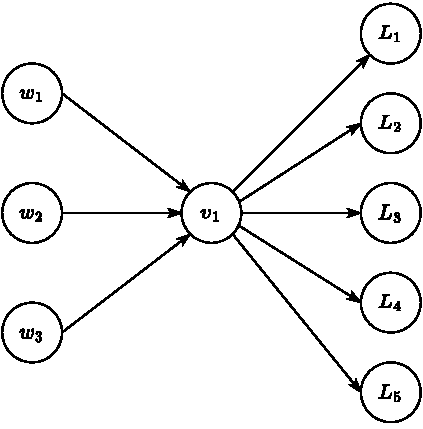
\includegraphics[width=1.82292in,height=\textheight,keepaspectratio]{ad_choose.pdf}

}

\caption{Какой режим вы бы выбрали для вычисления градиентов?}

\end{figure}%

\subsection{Задача 2}\label{ux437ux430ux434ux430ux447ux430-2}

Предположим, у нас есть обратимая матрица \(A\) и вектор \(b\), вектор
\(x\) является решением системы линейных уравнений \(Ax = b\), то есть
можно записать аналитическое решение \(x = A^{-1}b\).

\hfill\break
\hfill\break

\begin{tcolorbox}[enhanced jigsaw, colframe=quarto-callout-color-frame, rightrule=.15mm, toprule=.15mm, coltitle=black, opacityback=0, colback=white, leftrule=.75mm, arc=.35mm, opacitybacktitle=0.6, bottomrule=.15mm, breakable, toptitle=1mm, colbacktitle=quarto-callout-color!10!white, bottomtitle=1mm, title=\textcolor{quarto-callout-color}{\faInfo}\hspace{0.5em}{Question}, left=2mm, titlerule=0mm]

Найдите производные
\(\dfrac{\partial L}{\partial A}, \dfrac{\partial L}{\partial b}\).

\end{tcolorbox}

\begin{figure}[H]

{\centering 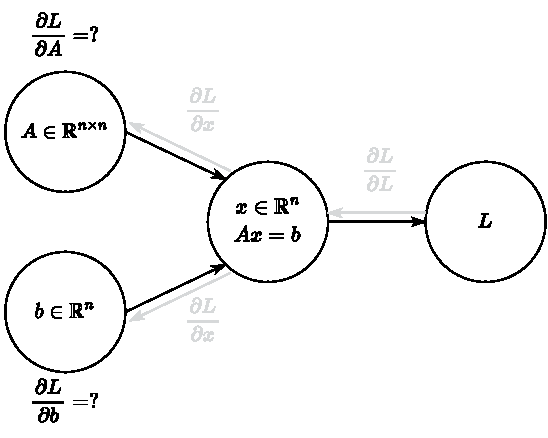
\includegraphics[width=2.08333in,height=\textheight,keepaspectratio]{linear_least_squares_layer.pdf}

}

\caption{\(x\) может быть найден как решение линейной системы}

\end{figure}%

\subsection{Задача 3}\label{ux437ux430ux434ux430ux447ux430-3}

Предположим, у нас есть прямоугольная матрица
\(W \in \mathbb{R}^{m \times n}\), которая имеет сингулярное разложение:

\hfill\break
\hfill\break

\[
W = U \Sigma V^T, \quad U^TU = I, \quad V^TV = I,
\] \[
\Sigma = \text{diag}(\sigma_1, \ldots, \sigma_{\min(m,n)})
\]

\hfill\break
\hfill\break
Регуляризатор \(R(W) = \text{tr}(\Sigma)\) в любой функции потерь
стимулирует низкоранговые решения.

\begin{tcolorbox}[enhanced jigsaw, colframe=quarto-callout-color-frame, rightrule=.15mm, toprule=.15mm, coltitle=black, opacityback=0, colback=white, leftrule=.75mm, arc=.35mm, opacitybacktitle=0.6, bottomrule=.15mm, breakable, toptitle=1mm, colbacktitle=quarto-callout-color!10!white, bottomtitle=1mm, title=\textcolor{quarto-callout-color}{\faInfo}\hspace{0.5em}{Question}, left=2mm, titlerule=0mm]

Найдите производную \(\dfrac{\partial R}{\partial W}\).

\end{tcolorbox}

\begin{figure}[H]

{\centering 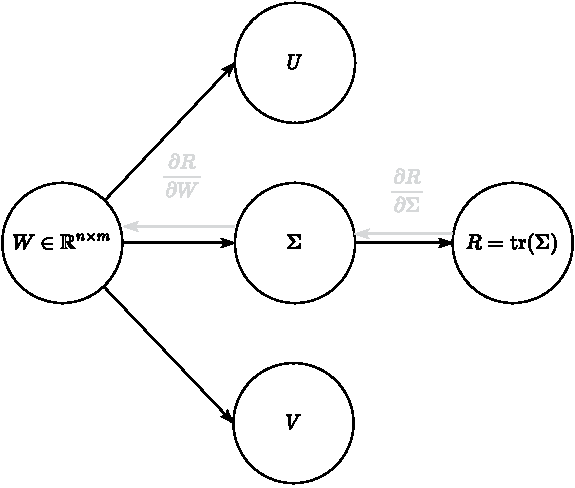
\includegraphics[width=2.08333in,height=\textheight,keepaspectratio]{svd_singular_regularizer_comp_graph.pdf}

}

\caption{Вычислительный граф для сингулярного регуляризатора}

\end{figure}%

\section{Задачи на
дом}\label{ux437ux430ux434ux430ux447ux438-ux43dux430-ux434ux43eux43c}

\begin{enumerate}
\def\labelenumi{\arabic{enumi}.}
\item
  \textbf{Бенчмаркинг вычисления произведения Гессиана на вектор (HVP) в
  нейронной сети через JAX} {[}22 балла{]}

  Вам дана простая нейронная сеть (MLP с несколькими скрытыми слоями с
  нелинейностью, такой как GELU). Параметры модели определяются весами
  ее слоев. Ваша задача состоит в том, чтобы сравнить различные подходы
  для вычисления произведения Гессиана на вектор (HVP) по отношению к
  функции потерь модели и изучить, как время вычисления масштабируется с
  ростом модели.

  \textbf{Определение модели и функции потерь:} {[}2/22 балла{]} Вот код
  для определения модели и функции потерь. Напишите метод
  \texttt{get\_params()}, который возвращает сглаженный вектор всех
  весов модели.

\begin{Shaded}
\begin{Highlighting}[]
\ImportTok{import}\NormalTok{ jax}
\ImportTok{import}\NormalTok{ jax.numpy }\ImportTok{as}\NormalTok{ jnp}
\ImportTok{import}\NormalTok{ time}
\ImportTok{import}\NormalTok{ matplotlib.pyplot }\ImportTok{as}\NormalTok{ plt}
\ImportTok{import}\NormalTok{ numpy }\ImportTok{as}\NormalTok{ np}
\ImportTok{import}\NormalTok{ pandas }\ImportTok{as}\NormalTok{ pd}
\ImportTok{from}\NormalTok{ tqdm.auto }\ImportTok{import}\NormalTok{ tqdm}
\ImportTok{from}\NormalTok{ jax.nn }\ImportTok{import}\NormalTok{ gelu}

\CommentTok{\# Определение MLP модели}
\KeywordTok{class}\NormalTok{ MLP:}
    \KeywordTok{def} \FunctionTok{\_\_init\_\_}\NormalTok{(}\VariableTok{self}\NormalTok{, key, layer\_sizes):}
        \VariableTok{self}\NormalTok{.layer\_sizes }\OperatorTok{=}\NormalTok{ layer\_sizes}
\NormalTok{        keys }\OperatorTok{=}\NormalTok{ jax.random.split(key, }\BuiltInTok{len}\NormalTok{(layer\_sizes) }\OperatorTok{{-}} \DecValTok{1}\NormalTok{)}
        \VariableTok{self}\NormalTok{.weights }\OperatorTok{=}\NormalTok{ [}
\NormalTok{            jax.random.normal(k, (layer\_sizes[i], layer\_sizes[i }\OperatorTok{+} \DecValTok{1}\NormalTok{]))}
            \ControlFlowTok{for}\NormalTok{ i, k }\KeywordTok{in} \BuiltInTok{enumerate}\NormalTok{(keys)}
\NormalTok{            ]}

    \KeywordTok{def}\NormalTok{ forward(}\VariableTok{self}\NormalTok{, x):}
        \ControlFlowTok{for}\NormalTok{ w }\KeywordTok{in} \VariableTok{self}\NormalTok{.weights[:}\OperatorTok{{-}}\DecValTok{1}\NormalTok{]:}
\NormalTok{            x }\OperatorTok{=}\NormalTok{ gelu(jnp.dot(x, w))}
        \ControlFlowTok{return}\NormalTok{ jnp.dot(x, }\VariableTok{self}\NormalTok{.weights[}\OperatorTok{{-}}\DecValTok{1}\NormalTok{])}

    \KeywordTok{def}\NormalTok{ get\_params(}\VariableTok{self}\NormalTok{):}
        \CommentTok{\#\#\# YOUR CODE HERE }\AlertTok{\#\#\#}
        \ControlFlowTok{return} \VariableTok{None}
\end{Highlighting}
\end{Shaded}

  \textbf{Гессиан и HVP:} {[}2/22 балла{]} Напишите функцию

\begin{Shaded}
\begin{Highlighting}[]
\CommentTok{\# Функция для вычисления Гессиана}
\KeywordTok{def}\NormalTok{ calculate\_hessian(model, params):}
    \KeywordTok{def}\NormalTok{ loss\_fn(p):}
\NormalTok{        x }\OperatorTok{=}\NormalTok{ jnp.ones((}\DecValTok{1}\NormalTok{, model.layer\_sizes[}\DecValTok{0}\NormalTok{]))  }\CommentTok{\# Заглушка входа}
        \ControlFlowTok{return}\NormalTok{ jnp.}\BuiltInTok{sum}\NormalTok{(model.forward(x))}

    \CommentTok{\#\#\# YOUR CODE HERE }\AlertTok{\#\#\#}
    \CommentTok{\#hessian\_fn =           }
    \ControlFlowTok{return}\NormalTok{ hessian\_fn(params)}
\end{Highlighting}
\end{Shaded}

  которая вычисляет полный Гессиан \(H\) функции потерь по отношению к
  параметрам модели с использованием автоматического дифференцирования
  JAX.

  \textbf{Naive HVP через полный Гессиан:} {[}2/22 балла{]} Напишите
  функцию \texttt{naive\_hvp(hessian,\ vector)}, которая, учитывая
  предварительно вычисленный Гессиан \(H\) и вектор \(v\) (той же формы,
  что и параметры), вычисляет произведение Гессиана на вектор с
  использованием прямого матрично-векторного умножения.

  \textbf{Эффективное HVP с использованием Autograd:} {[}4/22 балла{]}
  Напишите функцию
  \texttt{python\ \ \ def\ hvp(f,\ x,\ v):\ \ \ \ \ \ \ return\ jax.grad(lambda\ x:\ jnp.vdot(jax.grad(f)(x),\ v))(x)}
  которая непосредственно вычисляет HVP без явного формирования полного
  Гессиана. Это использует возможности обратного режима
  дифференцирования JAX.

  \textbf{Эксперимент по времени:} Рассмотрим семейство моделей с
  увеличивающимся количеством скрытых слоев.

\begin{Shaded}
\begin{Highlighting}[]
\NormalTok{ns }\OperatorTok{=}\NormalTok{ np.linspace(}\DecValTok{50}\NormalTok{, }\DecValTok{1000}\NormalTok{, }\DecValTok{15}\NormalTok{, dtype}\OperatorTok{=}\BuiltInTok{int}\NormalTok{)  }\CommentTok{\# The number of hidden layers}
\NormalTok{num\_runs }\OperatorTok{=} \DecValTok{10}  \CommentTok{\# The number of runs for averaging}
\end{Highlighting}
\end{Shaded}

  Для каждой конфигурации модели:

  \begin{itemize}
  \tightlist
  \item
    Сгенерируйте модель и извлеките ее вектор параметров.
  \item
    Сгенерируйте случайный вектор \(v\) той же размерности, что и
    параметры.
  \item
    Измерьте (не забудьте использовать \texttt{.block\_until\_ready()}
    для обеспечения точного измерения времени и правильной
    синхронизации) следующее:

    \begin{enumerate}
    \def\labelenumii{\arabic{enumii}.}
    \tightlist
    \item
      \textbf{Общее время (полный Гессиан + Naive HVP):} Общее время,
      необходимое для вычисления полного Гессиана и затем выполнения
      матрично-векторного умножения.
    \item
      \textbf{Время Naive HVP (без вычисления Гессиана):} Время,
      необходимое для выполнения матрично-векторного умножения, учитывая
      предварительно вычисленный Гессиан.
    \item
      \textbf{Время эффективного HVP:} Время, необходимое для вычисления
      HVP с использованием функции на основе autograd.
    \end{enumerate}
  \item
    Повторите каждое измерение времени для фиксированного количества
    запусков (например, 10 запусков) и запишите как среднее, так и
    стандартное отклонение времени вычисления.
  \end{itemize}

  \textbf{Визуализация и анализ:} {[}12/22 балла{]}

  \begin{itemize}
  \tightlist
  \item
    Постройте график результатов времени для трех методов на одном
    графике. Для каждого метода отобразите ошибки, соответствующие
    стандартному отклонению по запускам.
  \item
    Четко обозначьте оси (например, ``Количество слоев'' против ``Время
    вычисления (секунды)'') и включите легенду, указывающую, какая
    кривая соответствует какому методу.
  \item
    Анализируйте масштабирование. Попробуйте аналитически вывести
    масштабирование методов и сравнить его с экспериментальными
    результатами.
  \end{itemize}
\item
  {[}15 баллов{]} Мы можем использовать автоматическое дифференцирование
  не только для вычисления необходимых градиентов, но и для настройки
  гиперпараметров алгоритма, таких как скорость обучения в градиентном
  спуске (с градиентным спуском 🤯). Предположим, у нас есть следующая
  функция \(f(x) = \frac{1}{2}\Vert x\Vert^2\), выберите случайную точку
  \(x_0 \in \mathbb{B}^{1000} = \{0 \leq x_i \leq 1 \mid \forall i\}\).
  Рассмотрим \(10\) шагов градиентного спуска, начиная с точки \(x_0\):
  \[
   x_{k+1} = x_k - \alpha_k \nabla f(x_k)
   \] Ваша цель в этой задаче состоит в том, чтобы написать функцию,
  которая принимает \(10\) скалярных значений \(\alpha_i\) и возвращает
  результат градиентного спуска на функции \(L = f(x_{10})\). И
  оптимизируйте эту функцию с помощью градиентного спуска на
  \(\alpha \in \mathbb{R}^{10}\). Предположим, что каждый из \(10\)
  компонентов \(\alpha\) равномерно распределен на \([0; 0.1]\). \[
   \alpha_{k+1} = \alpha_k - \beta \frac{\partial L}{\partial \alpha}
   \] Выберите любую константу \(\beta\) и количество шагов, которое вам
  нужно. Опишите полученные результаты. Как вы поймете, что полученный
  график (\(\alpha \in \mathbb{R}^{10}\)) стал лучше, чем был в начале?
  Как вы проверите локальную оптимальность этой задачи численно?
\end{enumerate}




\end{document}
